%%%%%%%%%%%%%%%%%%%%%%%%%%%%%%%%%%%%%%%%
% Binary Relations and Orders
%%%%%%%%%%%%%%%%%%%%%%%%%%%%%%%%%%%%%%%%%%

\chapter{Binary Relations and Orders}

We define binary relations and orders on a collection of objects instead of on a set. This is because later we will define rewriting relations as binary relations, and the collection of objects subject to be rewritten in a rewriting system is not necessarily a set. For example, the collection of finite directed edge-labeled graphs is not a set, but a class.

\begin{notation}
    Let $C$ and $C'$ be collections of objects. We denote $c \mathop{\in} C$ for~\enquote{$c$ is an element of C}, $C \mathop{\cup} C'$ the smallest collection contains all elements in $C$ and all elements in $C'$, $C \mathop{\cap} C'$ the smallest collection contains all elements in $C$ that are also in $C'$, $C * C'$ the collection of ordered pairs with first element in $C$ and second element in $C'$.  
  \end{notation} 
  
  \begin{definition}[Binary relation]
    \label{def:binary_relation:binary_relation}
    Let $D$ be a collection of objects. A mathematical structure \( (D, \mathcal{R}) \) where $\mathcal{R}$ is a collection of objects from $D * D$ is called a \textbf{binary relation} on $D$. 
    
    For an object in $\mathcal{R}$ with first element $x \mathop{\in} D$ and second element $y\in D$, we write $x \mathcal{R} y$, $\mathcal{R}(x,y)$ or $(x,y) \mathop{\in} \mathcal{R}$. 
    
    When $D$ is irrelevant, we say simply that $\mathcal{R}$ is a binary relation.
  \end{definition} 
   
  \begin{definition}[Reflexivity,
    %  Antisymmetry, 
     Transitivity]
    \label{def:binary_relation:reflexivity_transitivity}
    A binary relation \( \mathop{\to} \) on \(C\) is said to be \textbf{reflexive} if for every object \(a \mathop{\in} C\), we have \(a \mathop{\to} a\); \textbf{transitive} if for all objects \( a, b, c \mathop{\in} C\), \( a \mathop{\to} b \mathop{\land} (b \mathop{\to} c) \) implies \(a \mathop{\to} c\).
  %       \item \textbf{antisymmetric} if \(
  % \forall a, b \mathop{\in} A, \, (a \mathop{\to} b) \mathop{\land} (b \mathop{\to} a) \implies a \mathop{=} b.
  % \)
  \end{definition}
  
  \begin{definition}[$\mathcal{R}$-sequence]
    \label{def:binary_relation:sequence}
    Let \(\mathcal{R}\) be a binary relation on $S$.
    A \textbf{\( \mathcal{R} \)-sequence} is either a finite sequence \( \left( s_i \right)_{0 \leq i \leq m} \) of elements in $S$ such that \(s_i \mathcal{R} s_{i+1}\) for each \( 0 \leq i \leq m-1\), or an infinite sequence \((s_i)_{i \mathop{\in} \mathbb{N}}\) of elements in $S$ such that \(s_n \mathcal{R} s_{n+1}\) for each \(i \mathop{\in} \mathbb{N}\).
\end{definition}

\begin{definition}[Well-founded binary relation]
    \label{def:binary_relation:well_founded}
    A binary relation $\to$ on a collection $S$ of object is said to be \textbf{well-founded} if there is no infinite $\to$-sequence. 
    % In other words, there does not exist an infinite sequence of elements $ (s_i)_{i \mathop{\in} \mathbb{N}} $ where $s_i \mathop{\in} S $ such that $s_i \mathop{\to} s_{i+1}$ for $i \mathop{\in} \mathbb{N}$.
\end{definition}

\begin{definition}[Transitive closure]
    \label{def:binary_relation:transitive_closure}
    The \textbf{transitive closure} of a binary relation $\to$, denoted $\to^+$, is the smallest transitive relation that include \( \mathop{\to} \).
  \end{definition}
  
  \begin{definition}[Reflexive-transitive closure]
    \label{def:binary_relation:reflexive_transitive_closure}
    The \textbf{reflexive transitive closure} of a binary relation $\to$, denoted $\to^*$, is the smallest reflexive and transitive relation that include \( \mathop{\to} \).
  \end{definition}

  \begin{definition}[Homomorphisms of binary relations]
    \label{def:binary_relation:homomorphism}
    Let $\to_\mathcal{A}$ be a binary relation on a collection $A$ of objects and $\to_\mathcal{B}$ be a binary relation on a collection $B$ of objects. A \textbf{homomorphism} from $\to_\mathcal{A}$ to $\to_\mathcal{B}$ is a function \( h: A \mathop{\to} B \) such that for all \( a, b \mathop{\in} A \), if \( a \mathop{\to} _\mathcal{A} b \) then \( h(a) \mathop{\to} _\mathcal{B} h(b) \).
  \end{definition}
  
\begin{proposition}[Proving well-foundedness]
  \label{prop:binary_relation:proving_well_foundedness}
  Let \(\to\) be binary relation and let $\leadsto$ be a well-founded binary relation. If there is a homomorphism from \(\to\) to \(\leadsto\), then \(\to\) is well-founded.
\end{proposition}
  
%%%%%%%%%%%%%%%%%%%%%%%%%%%%%%%%%%%%%%%%
%Rewriting relations and systems, and termination
%%%%%%%%%%%%%%%%%%%%%%%%%%%%%%%%%%%%%%%%%%

\chapter{Rewriting systems}
    \label{sec:category_of_rewriting_systems}      
      \begin{definition}[Rewriting relation]
        \label{def:ars}
        Let $D$ be a collection of objects.  
        A \textbf{rewriting relation} $(D, \rightarrow)$ on $D$ is defined as a binary relation on $D$.  
        The set $D$ is referred to as the \textbf{domain} of the rewriting relation.  
        For all objects $x, y \mathop{\in} D$, if $x \mathop{\rightarrow} y$ then we say that $x$ \textbf{rewrites} to $y$ (or there exists a \textbf{rewriting step} from $x$ to $y$).
    \end{definition}

      In the litterature, a rewriting relation is also called abstract rewriting systems or abstract reduction systems \cite{nipkow1998term,terese2003term} and is usually defined on a set of objects. We defined it on a collection of objects to cope with rewriting systems on graphs, which form a collection of objects but not a set.
       
      \begin{definition}[Rewriting system]
        \label{def:rewriting_system_no_framework}
        A \textbf{rewriting system} is defined as a mathematical structure $(D, \mathcal{R},M,W,\mathfrak{M},\mathfrak{W},\mathfrak{I})$ where 
        \begin{itemize}
          \item $D$ is a collection of objects. 
          \item $\mathcal{R}$ is a set of objects, called \textbf{rewriting rules},
          
          \item $M$ is a collection of objects, called \textbf{matches}, 
          
          \item $W$ is a collection of objects, called \textbf{witnesses of rewriting steps},  
          
          \item $\mathfrak{M}$ is a function, called \textbf{match mechanism}, which associates to each $(r,d) \mathop{\in} \mathcal{R} \mathop{\times} D$ a set $\mathfrak{M}(r,d)$ of matches in $M$, called \textbf{matches of the rewriting rule $r$ in the object $d$}, 
           
          \item $\mathfrak{W}$ is a function, called \textbf{witness function}, which associates to each $(r,d,m) \mathop{\in} \mathcal{R} \mathop{\times} D \mathop{\times} M$ a witness of rewriting step $\mathfrak{W}(r,d,m)$ in $W$, called \textbf{witness of the rewriting step defined by the match $m$ of the rule $r$ in the object $d$},

          \item $\mathfrak{I}$ is a function, called \textbf{interpretation function},  
              which associates to each witness $w \mathop{\in} W$, an element 
              in $D \mathop{\times} D$, called \textbf{rewriting step witnessed by $w$}.
        \end{itemize} 

        For every rule $\rho \mathop{\in} \mathcal{R}$, it induces a rewriting relation $\mathop{\Rightarrow}_\rho$ that is defined as follows: for all objects $s, t \mathop{\in} D$, the rewriting step $s \mathop{\Rightarrow}_\rho t$ exists
          iff there exists a match $m \mathop{\in} \mathfrak{M}(\rho,s)$ of the rule in the object $s$ such that $\mathfrak{W}(r,s,m)$ witnesses the rewriting step, i.e. $\mathfrak{I}(\mathfrak{W}(r,s,m)) \mathop{=} (s,t)$. 
          
          The \textbf{rewriting relation} $\mathop{\Rightarrow}_\mathcal{R}$ is defined as follows: for all objects $s, t \mathop{\in} D$, the rewriting step $s \mathop{\Rightarrow}_\mathcal{R} t$ exists iff $s \mathop{\Rightarrow}_\rho t$ for some rule $\rho \mathop{\in} \mathcal{R}$.

          For a rewriting step $s \mathop{\Rightarrow}_\rho t$ with match $m$, we denote $s \mathop{\Rightarrow}_\rho^m t$ to indicate the match $m$ used to rewrite $s$ to $t$.

          When the context makes it clear, we say that $\mathcal{R}$ is a rewriting system.
      \end{definition}
      
      When defining a rewriting system, one may want to impose additional constraints on the rewriting relation. This can be done by imposing a more restrictive match mechanism. 
      
      However, since rewriting is an intuitive concept, when we talk about a rewriting system on a given domain $D$, we have an intuition of what a match mechanism should be. 

      As a solution, Endrullis et al. proposed in \cite{endrullis2024generalized} to exclude certain witnesses using rewriting frameworks.
      
      \begin{definition}[Rewriting system in a rewriting framework]
        \label{def:rewriting_system_with_framework}
        A \textbf{rewriting system in a rewriting framework} is defined as a mathematical structure $(D, \mathcal{R},M,W,\mathfrak{M},\mathfrak{W},\mathfrak{I},\mathfrak{F})$ where
        \begin{itemize}
          \item $(\mathcal{R},M,W,\mathfrak{M},\mathfrak{W},\mathfrak{I})$ is a rewriting system,
          \item $\mathfrak{F}$ is a mapping, called \textbf{rewriting framework}, which associates to each rule $r \mathop{\in} R$, 
             a collection of witnesses in $W$.
        \end{itemize}
        
        For every rule $\rho \mathop{\in} \mathcal{R}$, it induces a rewriting relation $\mathop{\Rightarrow}_{\mathfrak{F},\rho}$ that is defined as follows: for all objects $s, t \mathop{\in} D$, the rewriting step $s \mathop{\Rightarrow}_{\mathfrak{F},\rho} t$ exists
          iff $s \mathop{\Rightarrow}_\rho^m t$ for some match $m \mathop{\in} \mathfrak{M}(\rho,s)$ and $\mathfrak{W}(r,s,m) \mathop{\in} \mathfrak{F}(\rho)$.

          The \textbf{rewriting relation} $\mathop{\Rightarrow}_{\mathfrak{F},\mathcal{R}}$ is defined as follows: for all objects $s, t \mathop{\in} D$, the rewriting step $s \mathop{\Rightarrow}_{\mathfrak{F},\mathcal{R}} t$ exists iff $s \mathop{\Rightarrow}_{\mathfrak{F},\rho} t$ for some rule $\rho \mathop{\in} \mathcal{R}$.

          For a rewriting step $s \mathop{\Rightarrow}_{\mathfrak{F},\rho} t$ with match $m$, we denote $s \mathop{\Rightarrow}_{\mathfrak{F},\rho}^m t$ to indicate the match $m$ used to rewrite $s$ to $t$.

          When the context makes it clear, we say that $\mathcal{R}$ is a rewriting system.
      \end{definition}
      
      % \trackedtext{useful ?? \\
      % The following correspond to the rewriting relation definition by rewriting framework proposed by Endrullis et Overbeek in \cite[Definition 5.2]{endrullis2024generalized}.
      % \begin{proposition}
      %   Let $D$ be a collection of objects.
      %   The structure $(\mathcal{R},\mathfrak{I},\mathfrak{F})$ where
      %   \begin{itemize}
      %     \item $\mathcal{R}$ is a set of objects, called \textbf{rewriting rules}, 
      %     \item $\mathfrak{F}$ is a function, called \textbf{rewriting framework},  which associates to each rule $r \mathop{\in} R$, 
      %        a class of objects,
      %     \item $\mathfrak{I}$ is a function, called \textbf{interpretation function},  
      %     which associates to each object $ w \mathop{\in} \mathcal{F}(r)$ with $r \mathop{\in} R$ an element 
      %     in $D \mathop{\times} D$, called \textbf{rewriting step using rule $r$ witnessed by $w$},
      %   \end{itemize}
      %    defines a rewriting relation $\to$ as follows: $ \mathop{\to} \mathop{=} \bigcup_{\rho \mathop{\in} R} \mathfrak{I}(\mathfrak{F}(\rho))$.
      % \end{proposition}
      % }
      
    % \color{red}


An abstract rewriting system is a mathcal structure in a first order language.
Intuitively, a mathcal structure is a set equipped with a binary relation on the set. 
A set is a collection of all elements that satisfy a certain given property. 
A binary relation on a set is a set of pairs of elements of that set. 
For more information on set theory, the reader is refer to \cite{jech2006set}. Bellow we give the formal definition these concepts.
  
\begin{definition}[Language~\text{\cite[Def 1.1.1]{marker2006model}}]
  A \textbf{language} \( \mathcal{L} \) is given by specifying the following data:
  \begin{itemize}
      \item  a set of function symbols \( \mathcal{F} \) and positive integers \( n_f \) for each \( f \in \mathcal{F} \);
      \item  a set of relation symbols \( \mathcal{R} \) and positive integers \( n_R \) for each \( R \in \mathcal{R} \);
      \item  a set of constant symbols \( \mathcal{C} \).
  \end{itemize}
\end{definition}

\begin{example}[\ \text{\cite{marker2006model}}]
  Consider the structure of the natural numbers with addition and distinguished elements 0 and 1. The natural language for studying this structure is the language where we have a binary function symbol for addition and constant symbols for 0 and 1. We would write sentences such as $\forall x \exists y (x = y + y \lor x = y + y +1)$, which we interpret as the assertion that “every number is either even or 1 plus an even number.”
\end{example}

\begin{definition}[Language of abstract rewriting systems]
  \label{def:l_ars}
  The first order \textbf{language of abstract rewriting systems} is $\mathcal{L}_\text{RS} = (\rightarrow)$ where $\rightarrow$ is a binary relation symbol.
\end{definition}
\begin{definition}[Structure~\text{\cite[Def 1.1.2]{marker2006model}}]
  An \( \mathcal{L} \)-\textbf{structure} \( \mathcal{M} \) is given by the following data:
 \begin{itemize}
     \item[i)] a nonempty set \( M \) called the \textit{universe, domain, or underlying set} of \( \mathcal{M} \);
     \item[ii)] a function \( f^{\mathcal{M}} : M^{n_f} \to M \) for each \( f \in \mathcal{F} \);
     \item[iii)] a set \( R^{\mathcal{M}} \subseteq M^{n_R} \) for each \( R \in \mathcal{R} \);
     \item[iv)] an element \( c^{\mathcal{M}} \in M \) for each \( c \in \mathcal{C} \).
 \end{itemize}
\end{definition}
We refer to \( f_{\mathcal{M}} \), \( R_{\mathcal{M}} \), and \( c_{\mathcal{M}} \) as the \textit{interpretations} of the symbols \( f \), \( R \), and \( c \). We often write the structure as \( \mathcal{M} = (M, f_{\mathcal{M}}, R_{\mathcal{M}}, c_{\mathcal{M}} : f \in \mathcal{F}, R \in \mathcal{R}, c \in \mathcal{C}) \). We will use the notation \( \mathcal{A}, \mathcal{B}, \mathcal{M}, \mathcal{N}, \dots \) to refer to the underlying sets of the structures \( A, B, M, N, \dots \).
\begin{definition}[Binary Relation]
  Let $S$ and $T$ be two sets. A \textbf{binary relation} from $S$ to $T$ is a subset of $S \times T$. A binary relation on $S$ is a binary relation from $S$ to $S$.
\end{definition} 

\begin{definition}[Abstract Rewriting System]
  \label{def:ars}
  An \textbf{rewriting system} is a $\mathcal{L}_\text{RS}$-structure $\mathcal{R} = (R,\to_\mathcal{R})$ where $R$ is a set and $\to_\mathcal{R}$ a binary relation on $R$. Elements $(x,y)$ in $\rightarrow_\mathcal{S}$, denoted $x \rightarrow_\mathcal{R} y$, will be called \textbf{rewriting steps}. 
\end{definition}

\begin{definition}[Reflexivity,
  %  Antisymmetry, 
   Transitivity]
  A binary relation \(\to \subseteq S\) is said to be
  \begin{itemize}
      \item \textbf{reflexive} if \(
          \forall a \in S, \, (a \to a)
          \)
%       \item \textbf{antisymmetric} if \(
% \forall a, b \in A, \, (a \to b) \land (b \to a) \implies a = b.
% \)
      \item \textbf{transitive} if \(
\forall a, b, c \in S, \, (a \to b) \land (b \to c) \implies (a \to c).
\)
  \end{itemize}
\end{definition}

\begin{definition}[Reflexive-Transitive Closure]
  The \textbf{reflexive transitive closure} of a binary relation $\to$, denoted $\to^*$, is the smallest reflexive and transitive relation that include \( \to \).
\end{definition}

\begin{definition}[Rewriting Relation]
   A rewriting system $\mathcal{R} = (R,\to_\mathcal{R})$ defines a \textbf{rewriting relation} $\to^{*}_{\mathcal{R}}$.
\end{definition}

\begin{definition}[Category of Rewriting Systems]
  Rewriting systems and homomorphisms between them form a category, denoted $\mathcal{RS}$.   
\end{definition}

\color{red}
\begin{definition}[Rewriting System Generated by Rewriting Rules in a Rewriting Framework]
  Let $A$ be a set and \( \mathfrak{F}: A \to \mathcal{P}(S^2) \) be a function.
  The rewriting system $\mathcal{S} = (S, \to_{\mathcal{S}})$ generated by the set of \textbf{rewriting rules} \( R \subseteq A \) within the \textbf{rewriting framework} \( \mathfrak{F}\) is defined by
  \[
      \to_\mathcal{S} = \bigcup_{\rho \in R} \mathfrak{F}(\rho)
    \]

  \todo{match mechanism:reviser}
  Let $M$ be a set, whose elements are called matches. Let \( \mathfrak{m}: R \times S \to \mathcal{P}(M) \) be a function such that for every \( (\rho,x) \in R \times S \), the set \( \mathfrak{m}(\rho, x) \) and the set $\{x \rightarrow_\mathcal{S} y \in \mathfrak{F}(\rho) \mid y \in S\}$ are in bijection. We say that \( \mathfrak{m} \) is a \textbf{match mechanism} and that elements in $\mathfrak{m}(\rho,x)$ are \textbf{matches} of the rule $\rho$ in the object $x$.

\end{definition}
\color{black}\color{black}
    \begin{definition}[Terminating rewriting relations]
        \label{def:rewriting_relation:termination}
    A rewriting relation is \textbf{terminating} if its transitive closure is well-founded.
    \end{definition}
    
    \begin{definition}[Terminating rewriting system]
        \label{def:rewriting_system:termination}
        A rewriting system 
        %  in a framework $\mathfrak{F}$ 
         is \textbf{terminating} if its rewriting relation
        %   $\to_{\mathcal{R},\mathfrak{F}}$ 
          is terminating.
    \end{definition}
    
    \begin{proposition}[Proving Termination of rewriting systems]
        Let $\mathcal{R}$ be a rewriting system and $\mathcal{S}$ be a terminating rewriting system.
        If there exists a homomorphism from the rewriting relation of $\mathcal{R}$ to the rewriting relation of $\mathcal{S}$, then $\mathcal{R}$ is terminating.  
    \end{proposition}
    
    In practice, it is often more convient to embed the rewriting system into a terminating rewriting system via a sequence of homomorphism.
    \begin{corollary}[Proving termination of rewriting systems]
      A rewriting system $\mathcal{R}$ is terminating if there is a terminating rewriting system $\mathcal{S}$ and homomorphisms $h_1,\ldots, h_n$ such that $h_n \circ \ldots \circ h_1$ is a homomorphism from $\mathcal{R}$ to $\mathcal{S}$.
    \end{corollary}
    
    \begin{definition}[Relative termination of rewriting relations]
        \label{def:rewriting_relation:relative_termination}
        Let \( \mathop{\to} \) and \( \leadsto \) be two rewriting relations. We say that \(\to\) is \textbf{terminating relative to} \(\leadsto\) if every \( \left( \mathop{\to} \mathop{\cup} \leadsto \right) \)-sequence contains only finitely many \(\to\)-steps.
    \end{definition}
    
    \begin{definition}[Relative termination of rewriting systems]
        \label{def:rewriting_system:relative_termination}
        Let $D$ be a collection of objects.
        Let \( \mathcal{A} \) and \( \mathcal{B} \) be two rewriting systems on $D$. We say that \(\mathcal{A}\) is \textbf{terminating relative to} \(\mathcal{B}\) if the rewriting relation induced by \(\mathcal{A}\) is terminating relative to the rewriting relation induced by \(\mathcal{B}\).
    \end{definition}
    
    % \begin{proposition}[Proving Relative Termination]
    %     Let \((S, \mathop{\to} \mathop{\cup} \leadsto) \) be an abstract rewriting system. \((S,\to)\) is \textbf{terminating relative to} \((S, \leadsto)\) if there is a terminating rewriting system $(R,>)$ and a function $h : S \mathop{\to} R$ such that
    %     \begin{itemize}
    %       \item $h$ is abstract rewriting system homomorphism from $(S,\to)$ to  $(R,>)$
    %       \item $h$ is abstract rewriting system homomorphism from $(S,\leadsto)$ to  $(R,\geq)$
    %     \end{itemize} 
    %     where $\geq$ is the reflexive closure of $>$.
    %   \end{proposition}
    \begin{definition}[Proving relative termination]
        \label{def:rewriting_system:proving_relative_termination}
        Let \( \mathcal{A} \) and \( \mathcal{B} \) be two rewriting systems on $D$. Let $>$ and $\geq$ be two rewriting relations on $D'$ such that $>$ is terminating relative to $\geq$. If there exists a function $h : D \mathop{\to} D'$ such that: (1) $h$ is a homomorphism from the rewriting relation of \(\mathcal{A}\) to $>$, and (2) $h$ is a homomorphism from the rewriting relation of \(\mathcal{B}\) to $\geq$, then \(\mathcal{A}\) is terminating relative to \(\mathcal{B}\).
    \end{definition}
    
    % \begin{definition}[Relative terminating rewriting systems]
    %     Let $D$ be a collection of objects.
    %     Let \( \mathcal{A} \) and \( \mathcal{B} \) be two rewriting systems on $D$.and $\mathfrak{F}$ be a DPO rewriting framework.
    %      We say that \(\mathcal{A}\) is \textbf{terminating relative to} \(\mathcal{B}\) if the rewriting relation \(\to_{\mathcal{A},\mathfrak{F}} \) is terminating relative to the rewriting relation \(\to_{\mathcal{B},\mathfrak{F}}\).
    % \end{definition}
    
    % \begin{definition}[Relative termination]
    % Let \((S, \mathop{\to} \mathop{\cup} \leadsto) \) be a rewriting system. We say that \((S,\to)\) is \textbf{terminating relative to} \((S, \leadsto)\) if every derivation $s_1 ( \mathop{\to} \mathop{\cup} \leadsto) s_2 ( \mathop{\to} \mathop{\cup} \leadsto) \hdots $ contains only finitely many $\to$-steps.
    % \end{definition} 
    
    % \color{red}
    % \begin{definition}[Pre-order \cite{davey2002introduction}]
    %   A reflexive and transitive binary relation $\geq$ on a set is called a pre-order. It give rise to a relation $>$ of strict inequality: $x \mathop{>} y$ iff $x \mathop{\geq} y$ and $x \mathop{\neq} y$. 
    % \end{definition} 
    
    % \begin{definition}[Partial Order]
    %   A reflexive, antisymmetric, transitive binary relation is called a partial order.
    % \end{definition}
    
    % \begin{definition}[Strict Partial Order]
    %   A irreflexive, transitive binary relation is called a strict partial order.
    % \end{definition}
    
    % \begin{example}[Lexicographic Product \cite{nipkow1998term}]
    %   Consider two rewriting systems $(A, >)$ and $(B, \mathop{\succ})$. The lexicographic product $(A \mathop{\times} B, \gg)$ is defined by the relation \((x,y) \gg (x',y')\) if and only if \(x \mathop{>} x'\) or, \(x \mathop{=} x'\) and \(y \mathop{\succ} y'\). If \(>\) and \(\mathop{\succ}\) are strict partial orders, then \(\gg\) is also a strict partial order. Furthermore, if both \((A, >)\) and \((B, \mathop{\succ})\) terminate, then the lexicographic product \((A \mathop{\times} B, \gg)\) will also terminate.
    % \end{example}
    
    % \begin{example}[Finite Lexicographic Product \cite{nipkow1998term}]
    %   By iteration, we can form lexicographic product over any number of rewriting systems $(A_i, >_i), i=1,\ldots,n$. For $n>1$, the lexicographic product $(A_1 \mathop{\times} (A_2 \mathop{\times} \ldots \mathop{\times} A_n),>_{1\ldots n})$ is the lexicographic product of $(A_1, >_1)$ and $(A_2 \mathop{\times} \ldots \mathop{\times} A_n,>{2\ldots n})$. Unwinding the recursion, we get 
    %   $(x_1,\ldots,x_n) >_{1\ldots n} (x_1',\ldots, x_n')$ iff $\exists k < n.(\forall i < k. x_i \mathop{=} x_i') \mathop{\land} x_k >_k x_k'$.
    %   If $(A_1,>_1), \ldots, (A_n,>_n)$ are strict partial orders, then so is $(A_1 \mathop{\times} \ldots \mathop{\times} A_n, >_{1\ldots n})$. 
    %   If $(A_1,>_1), \ldots, (A_n,>_n)$ terminates, then so does $(A_1 \mathop{\times} \ldots \mathop{\times} A_n, >_{1\ldots n})$. 
    % \end{example}
    
    % \begin{example}[Finite Lexicographic Product \cite{nipkow1998term}]
    %   A lexicographic product can be extended iteratively over any number of rewriting systems \((A_i, >_i)\) for \(i \mathop{=} 1, \ldots, n\). For \(n \mathop{>} 1\), the lexicographic product \((A_1 \mathop{\times} A_2 \mathop{\times} \dots \mathop{\times} A_n, >_{1\ldots n})\) is defined as the lexicographic product of \((A_1, >_1)\) and \((A_2 \mathop{\times} \dots \mathop{\times} A_n, >_{2\ldots n})\). Expanding this recursion, we have 
    %   \((x_1, \dots, x_n) >_{1\ldots n} (x_1', \dots, x_n')\) if and only if there exists \(k < n\) such that \((\forall i < k . x_i \mathop{=} x_i') \mathop{\land} x_k >_k x_k'\).
    %   If each \((A_1, >_1), \ldots, (A_n, >_n)\) is a strict partial order, then \((A_1 \mathop{\times} \dots \mathop{\times} A_n, >_{1\ldots n})\) is also a strict partial order. 
    %   Moreover, if \((A_1, >_1), \ldots, (A_n, >_n)\) terminate, then the lexicographic product \((A_1 \mathop{\times} \dots \mathop{\times} A_n, >_{1\ldots n})\) also terminates.
    % \end{example}
    
    
    % \begin{example}[Strings of Arbitrary but Finite Length with Lexicographic Order \cite{nipkow1998term}]
    %   Given an rewriting system \((A, >)\), the lexicographic order \((A^*, >_{lex})\) is defined as follows: \(x \mathop{>} x'\) if and only if \((|x| \mathop{>} |x'|) \lor (|x| \mathop{=} |x'| \mathop{\land} y \mathop{\succ} y')\).
    %   If \(>\) is a strict partial order, then \(\gg\) is also a strict partial order. Furthermore, if both \((A, >)\) and \((B, \mathop{\succ})\) are terminating rewriting systems, then their lexicographic product \((A \mathop{\times} B, \gg)\) also terminates.
    % \end{example}
    
    % \begin{definition}[Multiset Order \cite{nipkow1998term}]
    %   A \textbf{multiset} is a generalization of a set where elements can occur multiple times. Formally, it is defined as a function \( M: A \mathop{\rightarrow} \mathbb{N} \), where for each \(a \mathop{\in} A\), \(M(a)\) represents the number of times \(a\) appears in the multiset \(M\). The collection of all multisets over a set \(A\) is denoted by \(\mathcal{M}(A)\).
    
    %   Given a strict partial order \(>\) on a set \(A\), the corresponding multiset order \(>_{mul}\) on \(\mathcal{M}(A)\) is defined as follows: \(M >_{mul} N\) if and only if there exist multisets \(X, Y \mathop{\in} \mathcal{M}(A)\) such that:
    %   \begin{itemize}
    %       \item \(X \mathop{\subseteq} M\) and \(X \mathop{\neq} \emptyset\),
    %       \item \(N \mathop{=} (M - X) \mathop{\cup} Y\), and
    %       \item \(\forall y \mathop{\in} Y, \exists x \mathop{\in} X \text{ such that } x \mathop{>} y\).
    %   \end{itemize}
    %   If the rewriting system \((A, >)\) terminates, then the multiset order \((\mathcal{M}(A), >_{mul})\) also terminates.
    % \end{definition}
    % \color{black}
% In practice, it is often more convient to embed the rewriting system into a terminating rewriting system via a morphism that is the composition of a serie of morphisms.
% \begin{corollary}[Proving termination]
%   A rewriting system $\mathcal{R}$ is terminating if there is a terminating rewriting system $\mathcal{S}$ and functors $h_1,\ldots, h_n$ such that $h_1 \mathop{\star} \ldots \mathop{\star} h_n : \mathcal{R} \mathop{\to} \mathcal{S}$
% \end{corollary}

   
%   \begin{proposition}[Proving Relative Termination]
%     Let \((S, \mathop{\to} \mathop{\cup} \leadsto) \) be an abstract rewriting system. \((S,\to)\) is \textbf{terminating relative to} \((S, \leadsto)\) if there is a terminating rewriting system $(R,>)$ and a function $h : S \mathop{\to} R$ such that
%     \begin{itemize}
%       \item $h$ is abstract rewriting system homomorphism from $(S,\to)$ to  $(R,>)$
%       \item $h$ is abstract rewriting system homomorphism from $(S,\leadsto)$ to  $(R,\geq)$
%     \end{itemize} 
%     where $\geq$ is the reflexive closure of $>$.
%   \end{proposition}

%%%%%%%%%%%%%%%%%%%%%%%%%%%%%%%%%%%%%%%%%
% Graph Relabeling Systems
%%%%%%%%%%%%%%%%%%%%%%%%%%%%%%%%%%%%%%%%%%

\chapter{Graph Relabeling Systems}
    \label{sec:gls}
    \section{Graphs}
    \label{sec:graphs}
    \begin{definition}[Unlabeled graph~\cite{barr1990category}]
        \label{def:graph:unlabeled}
        An \textbf{unlabeled graph} \( G \) consists of a collection of \textbf{nodes} (also called \textbf{objects}) and a collection of \textbf{edges}, each equipped with a \textbf{source} (or \textbf{domain}) node and a \textbf{target} (or \textbf{codomain}) node. 
        For an unlabeled graph \( G \), we denote by \( G_0 \) its collection of nodes, \( G_1 \) its collection of edges, \( \operatorname{dom}:G_1{\to}G_0 \) the domain function, and \( \operatorname{cod}:G_1{\to}G_0 \) the codomain function. An unlabeled graph is \textbf{finite} if \( G_0 \) and \( G_1 \) are both finite sets.
        We write \( a: s \mathop{\to} t \) to indicate that \( a \) is a directed edge from \( s \) to \( t \). 
    \end{definition}   
    \begin{example}
      A unlabeled graph is a directed multigraph as illustrated below.
       
        \begin{center}
          \resizebox{0.45\textwidth}{!}{
          \begin{tikzpicture}
              \graphbox{\(\)}{00mm}{-20mm}{45mm}{20mm}{2mm}{-5mm}{
                  \coordinate (o) at (-5mm,-8mm); 
                  \node[draw,circle] (l1) at ($(o)+(-10mm,0mm)$) {};
                  % \node[draw,circle] (l2) at ($(l1)+(3,0)$) {};
                  \node[draw,circle] (l3) at ($(l1)+(1,0)$) {};
                  \node[draw,circle] (l4) at ($(l1)+(2,0)$) {};
                  \draw[->] (l1) edge[bend right]  (l3);
                  \draw[->] (l1) edge[bend left] (l3);
                  \draw[->] (l3) -- (l4);
                  % \draw[->] (l4) -- (l2) node[midway,above] {$a$};
              }  
          \end{tikzpicture}
      }
      \end{center} 
    \end{example}
    % A homomorphism of unlabeled graphs is a mapping between the nodes and edges of two graphs that preserves the graph structure.
    \begin{definition}
        \label{def:unlabeled_graph:homomorphism}
        Let \( G \) and \( H \) be unlabeled graphs. A \textbf{homomorphism of unlabeled graphs} $h: G \mathop{\to} H$ is a pair of functions $h_0: G_0 \mathop{\to} H_0 $ and $h_1: G_1 \mathop{\to} H_1$ such that for every edge \( a: s \mathop{\to} t \) in \( G \), we have \( h_1(a) : h_0(s) \mathop{\to} h_0(t) \) in \( H \).
    \end{definition}
    \begin{definition}
        \label{def:graph}
        Let \(\Sigma\) be a finite set of labels. A \textbf{labeled graph} is an ordered pair \((G,\lambda)\) where \( G \) is an unlabeled graph and \( \lambda : G_1 \mathop{\rightarrow} \Sigma\) is an edge-labeling function. 
        It is called \textbf{finite} if its underlying unlabeled graph is finite.  
    \end{definition}
    \begin{example} An labeled graph is edge-labeled directed multigraph as illustrated below.
       
        \begin{center}
          \resizebox{0.45\textwidth}{!}{
          \begin{tikzpicture}
              \graphbox{\( \)}{00mm}{-20mm}{45mm}{20mm}{2mm}{-5mm}{
                  \coordinate (o) at (-5mm,-8mm); 
                  \node[draw,circle] (l1) at ($(o)+(-10mm,0mm)$) {};
                  % \node[draw,circle] (l2) at ($(l1)+(3,0)$) {};
                  \node[draw,circle] (l3) at ($(l1)+(1,0)$) {};
                  \node[draw,circle] (l4) at ($(l1)+(2,0)$) {};
                  \draw[->] (l1) edge[bend right]  node[midway,below] {$a$} (l3);
                  \draw[->] (l1) edge[bend left] node[midway,above] {$a$}  (l3);
                  \draw[->] (l3) -- (l4) node[midway,above] {$b$};
                  % \draw[->] (l4) -- (l2) node[midway,above] {$a$};
              }  
          \end{tikzpicture}
      }
      \end{center} 
    \end{example}
    By $a : s\overset{l}{\rightarrow} t$, we denote the arrow $a$ labeled by $l$ from $s$ to $t$. Unless otherwise specified, the term \enquote{graph} refers to the graphs finite. Note that unlabeled graphs can be regarded as labeled graphs. 

    A homomorphism of labeled graphs is a homomorphism of unlabeled graphs that preserves the labels assigned to the edges.
    \begin{definition}
        \label{def:graph:homomorphism}
        Let \( (G,\lambda) \) and \( (H,\lambda') \) be labeled graphs. A \textbf{homomorphism of labeled graphs} $h:(G,\lambda) \mathop{\rightarrow} (H,\lambda')$ is a homomorphism of unlabeled graphs such that for each edge \( a \) in \( G \), we have \( \lambda (a) \mathop{=} \lambda' (h_1 (a)) \).
    \end{definition}
    \begin{notation}
        We use the notation from~\cite[Notation 1]{overbeek2023apbpotutorial} to visualize edge-labeled graph homomorphisms. Labeled graphs are enclosed in boxes with their names displayed in the top-left corner. Nodes and edges are assigned subsets of \(\mathbb{N}\) as identifiers, and these identifiers are chosen such that: (i) Each node or edge \( y \) in the codomain graph is assigned the union of the identifiers of all nodes or edges in the domain graph that are mapped to \( y \); (ii) The graph homomorphism is uniquely determined by this assignment.
        
        \noindent To further improve readability, we represent sets by listing their elements. Additionally, we omit identifiers when doing so does not cause confusion. Furthermore, if a node has a unique loop, we omit the loop and represent the corresponding label as a node-label. 
        This is illustrated in the following representation of a homomorphism \( h: G \mathop{\to} H \).
        
        \begin{center}
            \resizebox{0.45\textwidth}{!}{
            \begin{tikzpicture}
                \graphbox{\( G \)}{00mm}{-20mm}{45mm}{25mm}{2mm}{-10mm}{
                    \coordinate (o) at (-5mm,-8mm); 
                    \node[draw,circle] (l1) at ($(o)+(-10mm,0mm)$) {1};
                    \node[draw,circle] (l2) at ($(l1)+(3,0)$) {2};
                    \node[draw,circle] (l3) at ($(l1)+(1,0)$) {3};
                    \node[draw,circle] (l4) at ($(l1)+(2,0)$) {4};
                    \draw[->] (l1) -- (l3) node[midway,above] {$a$};
                    \draw[->] (l3) -- (l4) node[midway,above] {$b$};
                    \draw[->] (l4) -- (l2) node[midway,above] {$a$};
                }  
                \graphbox{\( H \)}{50mm}{-20mm}{34mm}{25mm}{2mm}{-10mm}{
                    \coordinate (o) at (0mm,-8mm); 
                    \node[draw,circle] (l1) at ($(o)+(-10mm,0mm)$) {1};
                    \node[draw,circle] (l2) at ($(l1)+(2,0)$) {2};
                    \node[draw,circle] (l3) at ($(l1)+(1,0)$) {3\ 4} node[above] {$b$};
                    \draw[->] (l1) edge node[midway,above] {$a$} (l3)  ;
                    % \draw[->] (l3) edge [loop above] node[midway,above] {$b$} (l3) ;
                    \draw[->] (l3) -- (l2) node[midway,above] {$a$};
                }      
                \node () at (48mm,-30mm) {$\rightarrow$};
            \end{tikzpicture}
        }
        \end{center} 
        In this example, the sets \(\{1\}\), \(\{2\}\), \(\{3\}\), \(\{4\}\), and \(\{3,4\}\) are represented as \(1\), \(2\), \(3\), \(4\), and \(3\ 4\), respectively. Edge identifiers are omitted.
    \end{notation} 

    \section{Graph Relabeling Systems (GRS)}
    \subsection{Graph Relabeling Systems (GLS)} 
Graph-relabeling-systems introduced in \cite{litovsky1999graph} are rewriting systems. For a given graph, a graph relabeling system identify a subgraph of the graph and modify the labels of the nodes and edges of this subgraph. Since it never modifies the structure of the graph, it is very intuitive.

% \begin{definition}[Graph Relabeling Rule]
%   A \emph{graph relabeling rule} is a couple of labeled graphs \( ((U,\lambda),(U, \lambda')) \) where \( (U, \lambda) \) is said to be the \emph{left-hand side graph} and \( (U, \lambda')\) the \emph{right-hand side graph}.
% \end{definition}  
\begin{definition}[GLS rewriting rule]
  \label{def:gls_rule}
  A \textbf{GLS rewriting rule} is an ordered pair of labeled graphs \( \rho \mathop{=} (U,\lambda) \mathop{\to} (U, \lambda') \) that share the same underlying unlabeled graph \( U \). The labeled graph \( (U, \lambda) \) is said to be the \textbf{left-hand side graph}, denoted $\opn{lhs}(\rho)$, and \( (U, \lambda')\) the \textbf{right-hand side graph}, denoted $\opn{rhs}(\rho)$.
\end{definition} 

\begin{example}
    \label{ex:gls_rule}
    The following is an example of a GLS rewriting rule. The left-hand side graph \( (U,\lambda) \) has two nodes labeled \( 1 \) and \( 2 \), and one edge labeled \( 0 \). The right-hand side graph \( (U,\lambda') \) has two nodes both labeled \( 1 \) and one edge labeled \( 1 \).
  \begin{center} 
    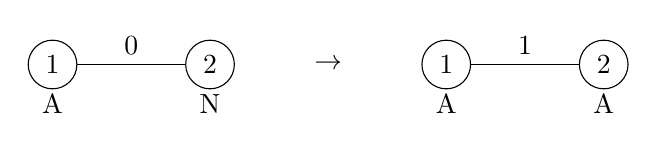
\begin{tikzpicture}
        % Left side
        \node[circle, draw] (A1) at (0,0) {1};
        \node[circle, draw] (N1) at (2,0) {2};
        \draw (A1) -- (N1) node[midway, above] {0};
        \node at (0,-0.5) {A};
        \node at (2,-0.5) {N};
    
        % Arrow
        \node at (3.5, 0) {$\rightarrow$};
    
        % Right side
        \node[circle, draw] (A2) at (5,0) {1};
        \node[circle, draw] (A3) at (7,0) {2};
        \draw (A2) -- (A3) node[midway, above] {1};
        \node at (5,-0.5) {A};
        \node at (7,-0.5) {A};
    \end{tikzpicture}
    \end{center}
\end{example}

% \begin{definition}[Match]
%   Let \(((U,\lambda),(U, \lambda')) \) be a graph relabeling rule. A \emph{match} of this rule in a labeled graph \( (G, \lambda_G) \) is a graph homomorphism \( m : (U,\lambda) \mathop{\to} (G, \lambda_G) \).
% \end{definition}

\todo{W est necessaire?}
\begin{definition}[Graph relabeling]
  \label{def:gls:rewriting}
  % \textbf{GLS match mechanism} is a mapping that associates to \( (\rho, G) \) the set of all injective graph homomorphisms $m : \opn{lhs}(\rho) \rightarrowtail G$.
 
  Let \( \rho \mathop{=} (L, \lambda_L) \mathop{\to} (R,\lambda_R) \) be a GLS rewriting rule, \( (G, \lambda_G) \) a graph.

  A \textbf{GLS match} of \( \rho \) in \( G \) is an injective graph homomorphism \( m : (L, \lambda_L) \rightarrowtail (G, \lambda_G) \). 
  
  Let $\lambda'_G$ be the labeling function on nodes and edges of \( G \) such that \( \lambda'_G(x) \mathop{=} \lambda_G(x) \) for all nodes and edges \( x \) in \( G \mathop{\setminus} \operatorname{Im}(m) \), and \( \lambda'_G(x) \mathop{=} \lambda_R(m^{-1}(x)) \) otherwise.

  Let $m' : (R, \lambda_R) \rightarrowtail (G, \lambda'_G)$ be the injective graph homomorphism with \( m(x) \mathop{=} m'(x) \) for all nodes and edges \( x \) in \( G \).

  The pair $(m, m')$ of injective graph homomorphisms is a \textbf{witness} of the rewriting step from \( (G, \lambda_G) \) to \( (G, \lambda'_G) \) using the rule \( \rho \) and match \( m \).
\end{definition}
\begin{definition}[Graph relabeling system]
  Let $\mathcal{R}$ be a set of GLS rewriting rules. Let $M, \mathfrak{M}, W , \mathfrak{W}, \mathfrak{I}$ be the match, match mechanism, witness, witness function and interpretation functions introduced in~\ref{def:gls:rewriting}.

  The structure $(\mathbf{Graph},\mathcal{R},M,W,\mathfrak{M},\mathfrak{W},\mathfrak{I})$ defines a rewriting system, called \textbf{graph relabeling system (GLS)}.
\end{definition}
\todo{example ref}
\begin{example}
  \label{example:gls_spinning_tree}
  Let \(\mathcal{R}\) be a graph relabeling system with labels in \( \{N, A, 0, 1\}\) a unique graph relabelling rule:

  \begin{center}
  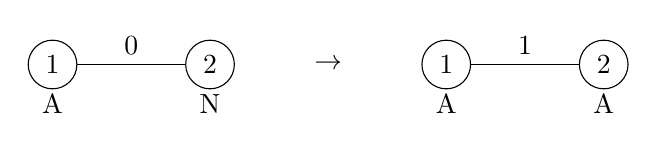
\begin{tikzpicture}
      % Left side
      \node[circle, draw] (A1) at (0,0) {1};
      \node[circle, draw] (N1) at (2,0) {2};
      \draw (A1) -- (N1) node[midway, above] {0};
      \node at (0,-0.5) {A};
      \node at (2,-0.5) {N};
  
      % Arrow
      \node at (3.5, 0) {$\rightarrow$};
  
      % Right side
      \node[circle, draw] (A2) at (5,0) {1};
      \node[circle, draw] (A3) at (7,0) {2};
      \draw (A2) -- (A3) node[midway, above] {1};
      \node at (5,-0.5) {A};
      \node at (7,-0.5) {A};
  \end{tikzpicture}
  \end{center}

  Let \( (G, \lambda) \) be a labeled graph such that all nodes are labeled \(N\) except for one node labeled \(A\), and all edges are labeled \(0\). 
  If we apply the rule \(r\) while it is possible, we obtain a labeled graph \( (G', \lambda') \) with all nodes labeled by \(A\) and all edges labeled by \(1\). Edges labeled by \(1\) in \( (G', \lambda') \) form a spanning tree of \( G \). 
\end{example}


    \subsection{Graph relabeling systems with priority relation on rules (PGLS)}
    Graph relabeling system with Priority is a graph relabeling system with a set of graph relabeling rules organized under a strict partial order. The priority mechanism ensures that certain rules are applied on certain area only when no higher-priority rules are applicable. This restriction depends on the order on the rules, and thus cannot be achieved by restricting the matching mechanism. In this section, we proposed to restrict the definition of a relabeling system via a rewriting framework.

 

    \begin{definition}
    \end{definition}
    
    \begin{definition}[Graph relabeling system with priority relation on rules]
      \label{def:pgls_framework}
    
      Let $\mathcal{R}$ be a set of graph relabeling rules and $<$ a strict partial order on $\mathcal{R}$.
    
      We defined a rewriting framework, denoted $\mathfrak{pgls}(\mathcal{R},<)$, as follows: for all $\rho \mathop{\in} \mathcal{R}$,
      $\mathfrak{pgls}(\mathcal{R},<)(\rho)$ is the classe of all witnesses of rewriting steps
      $\left(  m_\rho, m'_\rho \right)$ using the rule $\rho$
      such that there does not exist 
      a rule $\sigma \mathop{\in} \mathcal{R}$ with $\sigma \mathop{>} \rho$ and a witness of a rewriting step
      $\left(  m_\sigma, m'_\sigma \right)$ using the rule $\sigma$ such that 
      $\operatorname{Im}(m_\rho) \mathop{\cap} \operatorname{Im}(m_\sigma) \mathop{\neq} \emptyset$.
 
      The structure $(\mathbf{Graph},\mathcal{R},M,W,\mathfrak{M},\mathfrak{W},\mathfrak{I}, \mathfrak{pgls}(\mathcal{R},<))$, where $M, \mathfrak{M}, W , \mathfrak{W}, \mathfrak{I}$ are the match, match mechanism, witnesses, witness function and interpretation functions introduced in Definition~\ref{def:gls:rewriting}, defines a rewriting system, called \textbf{graph relabeling system with priority relation on rules (PGLS)}. 

    \end{definition}
     
     
    \todo{example: ref,  explanation}
    \begin{example}
      \label{example:pgrs_spanning_tree}
      Consider the GRS \(\mathcal{R}= \{r_1,r_2\}\) with \(\Sigma \mathop{=} \{N, A, 0, 1\}\) and \(r_1 \mathop{>} r_2\). The rules \(r_1\) and \(r_2\) are depicted below:
      
      \begin{tikzpicture}
      \draw (-1,0) node[left] {$r_1$:};
      
      \node[draw,circle] (x_1) at (0,0) {$1$};
      \draw (0,0.3) node[above]{A};
      \node[draw,circle, minimum size \mathop{=} 1pt] (x_2) at (2,0) {$2$};
      \draw (2,0.3) node[above]{N};
      \draw[-] (x_1) -- (x_2);
      
      \draw (3,0) node[right] {$\longrightarrow$};
      
      \node[draw,circle] (x3) at (5,0) {$1$};
      \draw (5,0.3) node[above]{M};
      \node[draw,circle, minimum size \mathop{=} 1pt] (x4) at (7,0) {$2$};
      \draw (7,0.3) node[above]{A};
      \draw[-] (x3) -- (x4);
      \end{tikzpicture}
      
      \begin{tikzpicture}
      \draw (-1,0) node[left] {$r_2$:};
      
      \node[draw,circle] (x_1) at (0,0) {$1$};
      \draw (0,0.3) node[above]{M};
      \node[draw,circle, minimum size \mathop{=} 1pt] (x_2) at (2,0) {$2$};
      \draw (2,0.3) node[above]{A};
      \draw[-] (x_1) -- (x_2);
      
      \draw (3,0) node[right] {$\longrightarrow$};
      
      \node[draw,circle] (x3) at (5,0) {$1$};
      \draw (5,0.3) node[above]{A};
      \node[draw,circle, minimum size \mathop{=} 1pt] (x4) at (7,0) {$2$};
      \draw (7,0.3) node[above]{F};
      \draw[-] (x3) -- (x4);
      \end{tikzpicture}
    \end{example}
     
    \subsection{Graph relabeling systems with Forbidden Contexts (FCGLS)}
    \begin{itemize}
        \item 03/22 : fcgls modifies the match mechanism
      \end{itemize}
      
      This section explores Graph Relabeling Systems with Forbidden Contexts (FCGLS), where each relabeling rule is constrained by specific contexts in which it cannot be applied. These forbidden contexts are defined by a function that associates each rule with a set of morphisms, ensuring that the rule is only applied when certain conditions are met. This approach adds a layer of control to the rewriting process, preventing certain transformations from occurring in undesired situations.
     
      \cite{litovsky1999graph}
      
      \begin{definition}[Graph rewriting framework with forbidden contexts on rules]
        Let $\mathcal{R}$ be a finit set of GLS rewriting rules and $f$ a function associating to every rule $(L \mathop{\rightarrow} R) \mathop{\in} \mathcal{R}$ a finite set of graph homomorphisms from $L$.
      
        We define a rewriting framework, denoted $\mathfrak{fcgls}(\mathcal{R},f)$, as follows: for $\rho \mathop{=} (L \mathop{\rightarrow} R) \mathop{\in} \mathcal{R}$, $\mathfrak{fcgls}(\mathcal{R},f)(\rho)$ is the classe of all GLS witnesses of rewriting steps
        $\left(  m: L \rightarrowtail G, m'  \right)$ such that 
      
        for all $(h : L \rightarrowtail F) \mathop{\in} f(\rho)$, there is no $g:F \rightarrowtail G$ such that $h \mathop{\star} g \mathop{=} m$.
      \end{definition}

      
      \begin{definition}[Graph relabeling system with Forbidden Contexts]
        Let $\mathcal{R}$ be a set of GLS rewriting rules and $f$ a function associating to every rule $(L \mathop{\rightarrow} R) \mathop{\in} \mathcal{R}$ a finite set of graph homomorphisms from $L$.

        Let $M, \mathfrak{M}, W , \mathfrak{W}, \mathfrak{I}$ be the match, match mechanism, witness, witness function and interpretation functions introduced in Definition~\ref{def:gls:rewriting}.
      
        The structure $(\mathbf{Graph},\mathcal{R},M,W,\mathfrak{M},\mathfrak{W},\mathfrak{I}, \mathfrak{fcgls}(\mathcal{R},f))$ defines a rewriting system, called \textbf{graph relabeling system with forbidden contexts (FCGLS)}. 
      \end{definition} 
      
        \todo{prop: ref,prop: def: equivalence}
      \begin{proposition}
        The PGRSs and the FCGRSs are equivalent.
      \end{proposition}
      \begin{example}[Distributed Computation of a Spanning Tree With Local Detection of the Global Termination \text{\cite[Example 14]{litovsky1999graph}}]
      \label{example:fcgls_spanning_tree}
      
      
       Consider the graph relabelling system $\mathcal{R}$ which constructs a spanning tree when it 
      terminates. Initial graphs have all edges labelled by $0$, and all vertices labelled by $N$ but one 
      vertex labelled by $A$. The set of labels is $\{A, A',N,0,1,F \}$. The set of relabelling rules are
      
                    
                \begin{tikzpicture}
                    \draw (-1,0) node[left] {$r_1$:};
                    \draw (1,0) node[above] {0};
                    
                    \node[draw,circle] (x_1) at (0,0) {} ;
                    \draw (0,0.1) node[above]{A};
                    \node[draw,circle] (x_2) at (2,0) {};
                    \draw (2,0.1) node[above]{N};
                    \draw[-] (x_1) -- (x_2);
                    
                    \draw (3,0) node[right] {$\longrightarrow$};
                    \draw (6,0) node[above] {1};
                    
                    \node[draw,circle] (x3) at (5,0) {} ;
                    \draw (5,0.1) node[above]{A};
                    \node[draw,circle] (x4) at (7,0) {};
                    \draw (7,0.1) node[above]{A'};
                    \draw (7.5,-0.45) node[above]{$,$};
                    \draw (8,-0.45) node[above]{$\Big\{$};
                    \draw (8.5,-0.45) node[above]{$\Big\}$};
                    \draw[-] (x3) -- (x4);
                \end{tikzpicture}
                
                
                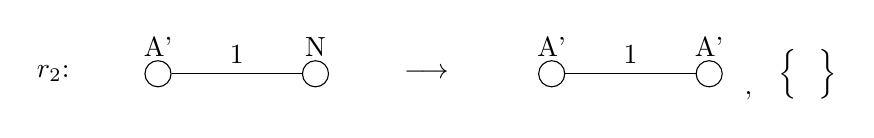
\begin{tikzpicture}
                    \draw (-1,0) node[left] {$r_2$:};
                    \draw (1,0) node[above] {1};
                    
                    \node[draw,circle] (x_1) at (0,0) {} ;
                    \draw (0,0.1) node[above]{A'};
                    \node[draw,circle] (x_2) at (2,0) {};
                    \draw (2,0.1) node[above]{N};
                    \draw[-] (x_1) -- (x_2);
                    
                    \draw (3,0) node[right] {$\longrightarrow$};
                    \draw (6,0) node[above] {1};
                    
                    \node[draw,circle] (x3) at (5,0) {} ;
                    \draw (5,0.1) node[above]{A'};
                    \node[draw,circle] (x4) at (7,0) {};
                    \draw (7,0.1) node[above]{A'};
                    \draw (7.5,-0.45) node[above]{$,$};
                    \draw (8,-0.45) node[above]{$\Big\{$};
                    \draw (8.5,-0.45) node[above]{$\Big\}$};
                    \draw[-] (x3) -- (x4);
                \end{tikzpicture}
      
      
                \begin{tikzpicture}[scale \mathop{=} 0.8]
                    \draw (-1,0) node[left] {$r_3$:};
                    
                    \node[draw,circle] (x_1) at (0,0) {1} ;
                    \draw (0,0.4) node[above]{A'};
                    
                    \draw (1,0) node[right] {$\longrightarrow$};
                    
                    \node[draw,circle] (x3) at (3,0) {1} ;
                    \draw (3,0.1) node[above]{F};
                    
                    %context 1
                    \node[draw,circle](c1_1) at (5,0.75) {$1$};
                    \draw (5,1.1) node[above] {A'};
                    \node[draw,circle](c1_2) at (5,-0.75){$2$};
                    \draw (5,-1.1) node[below] {N};
                    \draw (5,0) node[left] {$0$};
                    \draw[-] (c1_1)--(c1_2);
                    \draw (5.5,-0.45) node[above]{$,$};
                    
                    %context 2
                    \node[draw,circle](c2_1) at (7,0.75) {$1$};
                    \draw (7,1.1) node[above] {A'};
                    \draw (6.25,-1.1) node[below] {A'};
                    \draw (7.75,-1.1) node[below] {A'};
                    \node[draw,circle](c2_2) at (6.25,-0.75) {$3$};
                    \node[draw,circle](c2_3) at (7.75,-0.75) {$4$};
                    \draw[-] (c2_1) -- (c2_2);
                     \draw (6.6,0) node[left] {$1$};
                    \draw (7.35,0) node[right] {$1$};
                    \draw[-] (c2_1) -- (c2_3);
                    \draw (8,-0.45) node[above]{$,$};
                    
                    %context 3
                    \node[draw,circle](c3_1) at (9.25, 0.75) {$1$};
                    \node[draw,circle](c3_2) at (8.75, -0.75) {$5$};
                    \node[draw,circle](c3_3) at (9.75, -0.75) {$6$};
                    \draw (9.25,1.1)     node[above] {A'};
                    \draw (8.75,-1.1) node[below] {A'};
                    \draw (9.75,-1.1) node[below] {A};
                    \draw (9,0) node[left] {$1$};
                    \draw (9.5,0) node[right] {$1$};
                    \draw[-] (c3_1) -- (c3_2);
                    \draw[-] (c3_1) -- (c3_3);
                    
                    
                    \draw (3.5,-0.45) node[above]{$,$};
                    \draw (4,-0.45) node[above]{$\Big\{$};
                    \draw (10.5,-0.45) node[above]{$\Big\}$};
                \end{tikzpicture}
      \end{example}
      
      % \begin{definition}[FCGLS \cite{litovsky1999graph} ]
      %   \todo[tickmarkheight=0.1cm]{todo}
      % Let $(G,\lambda)$ be a labelled graph. A context of $(G,\lambda)$ is a triple $(H,\mu,\psi)$
      %  such that $(H,\mu)$ is a labelled graph and $\psi$ an occurrence of $(G,\lambda)$ in $(H,\mu)$.
          
      % A relabelling rule with forbidden contexts is a 4-tuple $R=(G_R,\lambda_R,\lambda'_R,F_R)$ such 
      % that $(G_R,\lambda_R,\lambda'_R)$.
          
      % A graph relabelling system with forbidden contexts (FCGRS) is a triple $\mathcal{R} \mathop{=} (L,I,P)$ 
      % defined as a GRS except that the set P is a set of relabelling rules with forbidden contexts. 
      % \end{definition}
      
      
      % \begin{definition}[Graph Relabeling System With priorities and Forbidden Contexts \cite{litovsky1999graph}]
      %   Let $\mathcal{R}$ be a set of graph relabeling rules,  $>$ a strict partial order on $\mathcal{R}$, and $f$ a function associating to every rule $r$ a set of morphisms from $lhs(r)$ in \textbf{Graph}.  For all labeled graph $H$, for all $r\mathcal{R}$, let  
      %   \begin{flalign*}
      %     \f{F}_{fcpgls}(r) \isdef 
      %     \f{F}_{pgls}(r) \mathop{\cap} \f{F}_{fcgls}(r)
      %   \end{flalign*}
      %   The rewriting system $(\textbf{Graph}, \mathop{\to} _\mathcal{R})$, générated by $\mathcal{R}$ and $\f{F}_{fcpgls}$ is called a \textbf{graph relabeling system with priorities and forbidden contexts} (FCPGLS).
      % \end{definition}
       
      % Let $G,G'$ be two graphs. A \textbf{graph homomorphism} consists of two functions $h_0 : G_v \mathop{\to} G_v'$ and $h_1: G_e \mathop{\to} G_e'$ such that 
      % for all $x \mathop{\in} G_e$
      % \begin{itemize}
      %       \item $G'_s( h_1(x)) \mathop{=} h_0(G_s(x))$ 
      %       \item $G'_t( h_1(x)) \mathop{=} h_0(G_t(x))$  
      %       \item $G'_l( h_1(x)) \mathop{=} G_l(x)$   
      % \end{itemize}
      
       
    \section{Termination}
    \todo{useful?}
    \color{red}
      When the set $\Sigma$ of labels is finite, it is decidable whether a graph relabeling system is terminating.
    , it is possible to determine whether all reduction sequences starting from a given graph will eventually terminate. 
    
    \begin{proposition}
      Let $\Sigma$ be a finite set of labels.  Let $\mathcal{R}$ be a graph relabeling system, a graph relabeling system with priorities or a graph relabeling system with forbidden contexts. The termination of $(\textbf{Graph}, \mathop{\to} _{\mathfrak{gls(\mathcal{R})}})$ is decidable.
      \end{proposition}
      \begin{proof}
         Since the graph relabeling rules donnot modify the underlying unlabeled graph and the set of labels and the set of rules are finite, the set of accessible graphs from $G$ is finite. Furthermore, there are only finite possible rewriting sequences. If there is a rewriting sequence which has a cycle, then the graph relabeling system is not terminating, otherwise it terminates.
      \end{proof}
    
    \begin{remark}
      It is infeasible to check all rewriting sequence from all graphs.
    \end{remark}
    \color{black}

\chapter{First Order Term Rewriting Systems}
    \label{sec:trs} 
    
\section{Terms}
Terms on which first order term rewriting systems are defined are terms of a first order language.
% \begin{definition}[Signature $\Sigma$~\cite{nipkow1998term}]
%   A \textbf{signature} \( \Sigma \) is a set of function symbols and for each \( f \mathop{\in} \Sigma \) a non-negative integer \( n \) called the arity of \( f \).
% \end{definition}
\begin{definition}[First order language~\text{\cite[Def 1.1.1]{marker2006model},\cite[Def 2.1.1]{terese2003term}}]
  A \textbf{language} \( \mathcal{L} \) is given by specifying the following data:
  \begin{itemize}
      \item  a set of function symbols \( \mathcal{F} \) and positive integers \( n_f \) for each \( f \mathop{\in} \mathcal{F} \);
      \item  a set of relation symbols \( \mathcal{R} \) and positive integers \( n_R \) for each \( R \mathop{\in} \mathcal{R} \);
      \item  a set of constant symbols \( \mathcal{C} \).
  \end{itemize}
\end{definition}
% \begin{definition}[$\Sigma$-Terms]
%   Let $\Sigma$ be a signature. The set $T(\Sigma)$ of $\Sigma$-terms is the smallest set such that 
%   \begin{itemize}
%     \item for all $n\geq 0$, all function symbols $f$ of arity n, and all $t_1,\hdots, t_n \mathop{\in} T(\Sigma, \mathcal{X})$, we have $f(t_1,...,t_n) \mathop{\in} T(\Sigma, \mathcal{X})$.
%   \end{itemize}
% \end{definition}

\begin{definition}[$(\Sigma,\mathcal{X})$-Terms~\text{\cite{nipkow1998term},\cite[Def 2.1.2]{terese2003term}}]
  Let $\Sigma$ be a first order language and $\mathcal{X}$ be a countably infinite set of variable symbols such that $\Sigma \mathop{\cap} \mathcal{X} \mathop{=} \emptyset$. The set $T(\Sigma,\mathcal{X})$ of $(\Sigma,\mathcal{X})$-terms is the smallest set such that 
  \begin{itemize}
  \item $\mathcal{X} \mathop{\subseteq} T(\Sigma,\mathcal{X})$, and
  \item for all $n\geq 0$, all function symbols $f$ of arity n, and all $t_1,\hdots, t_n \mathop{\in} T(\Sigma, \mathcal{X})$, we have $f(t_1,...,t_n) \mathop{\in} T(\Sigma, \mathcal{X})$.
  \end{itemize}
\end{definition}


\section{Term Rewriting Systems}

\subsection{TRS}
A term rewriting system (TRS) is a rewriting system where the objects are $T(\Sigma,\mathcal{X})$-terms where $\Sigma$ is a set of function symbols and $\mathcal{X}$ is a set of variable symbols disjoint from $\Sigma$.
  
\begin{definition}[term rewriting rule~\text{\cite[Def.2.2.1]{terese2003term}}]
    Let $\Sigma$ be a first order language and $\mathcal{X}$ be a set of variables. A \textbf{term rewriting rule} is an ordered pair $(l,r) \mathop{\in} T(\Sigma, \mathcal{X})^2$, denoted $l \mathop{\to} r$, such that
    \begin{itemize}
      \item $l$ is not a variable, and
      \item every variable occurring in $r$ also occurs in $l$.
    \end{itemize}
  \end{definition}
  
  \begin{definition}[Position \cite{nipkow1998term} \cite{urbain2001approche}]
    Let $\Sigma$ be a first order language and $\mathcal{X}$ be a set of variable symbols disjoint from $\Sigma$. Let $s \mathop{\in} T(\Sigma, \mathcal{X})$.
    The set of positions of subterms of $s$ is a set $\operatorname{Pos}(s)$ defined by induction as follows:
    \begin{itemize}
      \item if $s \mathop{\in} \mathcal{X}$, then $\operatorname{Pos}(s) \mathop{=} \set{\epsilon}$
      \item if $s \mathop{=} f(t_1,\hdots,t_n)$, 
            then $\operatorname{Pos}(s) \mathop{=} \set{\epsilon} \mathop{\cup} \bigcup_{1 \leq k \leq n} \left \{kp\mid p \mathop{\in} \operatorname{Pos}(t_k) \right \}$
  \end{itemize}
  A position of a subterm of $s$ is a word on alphabet $\mathbb{N}\mathop{\setminus}\set{0}$. 
    The concatenation of words $p$ and $q$ will be denoted $pq$.
  \end{definition}

  \begin{definition}[Subterm \cite{nipkow1998term} \cite{urbain2001approche}]
    For $p \mathop{\in} \mathcal{Pos}(s)$, the \textbf{subterm of s at position p}, denoted by $s_{|p}$, is defined by induction on the length of p:
    \begin{itemize}
      \item $s_{|\epsilon} := s$, and
      \item $f(s_1,...,s_n)_{|iq} := \left(s_i\right)_{|q}$.
    \end{itemize} 
    
    Note that, for $p \mathop{=} iq$, $p \mathop{\in} \mathcal{Pos}$ implies that s is of the form $s \mathop{=} f(s_1,...,s_n)$ with $i \le n$
    
    For $p \mathop{\in} \mathcal{Pos}(s)$, we denote by $s[t]_p$ the term that is obtained from s by \textbf{replacing the subterm at position p by t}:
  \begin{itemize}
    \item $s[t]_\epsilon := t$
    \item $f(s_1,...,s_n)[t]_{iq} := f(s_1,...,s_i[t]_{q},...,s_n)$
  \end{itemize}
 
  \end{definition}
   
  \begin{definition}[Substitution]
    Let $\Sigma$ be a first order language and $\mathcal{X}$ be a set of variables.
    A \text{substitution} is a function $\sigma : \mathcal{X} \mathop{\rightarrow} T(\Sigma, \mathcal{X})$ such that $\sigma(x) \not \mathop{=} x$ for only finitely many variables. Any substitution can be extended to a mapping on $T(\Sigma,\mathcal{X})$ by letting $\sigma(f(s_1,...,s_n)) \overset{\operatorname{def}}{=}f(\sigma(s_1),...,\sigma(s_n))$.
  \end{definition}

   
  \begin{definition}[Term rewriting]
    \label{def:trs:rewriting}
    Let $\Sigma$ be a first order language and $\mathcal{X}$ be a set of variables. Let $\mathcal{R}$ be a set of TRS rewriting rules. Let $s \mathop{\in} T(\Sigma, \mathcal{X})$ and $\rho \mathop{=} (l \mathop{\to} r) \mathop{\in} \mathcal{R}$. Let $p$ be a match of $\rho$ in $s$.

      A \textbf{match} of $\rho$ in $s$ is a position $p \mathop{\in} \operatorname{Pos}(s)$ such that there exists a substitution $\sigma$ such that $s_{|p} \mathop{=} \sigma(l)$.

    The triple $(\rho, s, p, \sigma)$ is a witness of the rewriting step $s \mathop{\to} _\rho^p t$ where $t \mathop{=} s[\sigma(r)]_p$.
  \end{definition}
  
  \begin{definition}[TRS rewriting system]
    Let $\mathcal{R}$ be a set of TRS rules. 

    Let $M, \mathfrak{M}, W , \mathfrak{W}, \mathfrak{I}$ be the match, match mechanism, witnesses, witness function and interpretation functions introduced in Definition~\ref{def:trs:rewriting}
 
    The rewriting system $(T(\Sigma,\mathcal{X}), \mathcal{R}, M, \mathfrak{M}, W, \mathfrak{W}, \mathfrak{I})$ is called a \textbf{term rewriting system (TRS)}.
  \end{definition}

  % \begin{definition}[Term Rewriting System]
  %   Let $\Sigma$ be a signature and $\mathcal{X}$ be a set of variables.
  %   Let $\mathcal{R} \mathop{\subseteq} T(\Sigma,\mathcal{X})^2$.
  %   For all $s \mathop{\in} T(\Sigma, \mathcal{X})$ and for all $l \mathop{\to} r \mathop{\in} \mathcal{R}$ we define
  %   % \begin{flalign*}
  %   %   \operatorname{Acc}_{trs}(s,l \mathop{\to} r) \overset{\operatorname{def}}{=} 
  %   %     \left \{ 
  %   %         s[\sigma(r)]_p \mid p \mathop{\in} \operatorname{Pos}(s) \mathop{\land} \exists \sigma. s|_p \mathop{=} \sigma(l)
  %   %       \right \}
  %   % \end{flalign*}
  %   \begin{flalign*}
  %     \f{F}_{trs}(l \mathop{\to} r) \overset{\operatorname{def}}{=} 
  %       \left \{ 
  %           (s,t) \mid 
  %             \exists C \mathop{\in} T(\Sigma \mathop{\cup} \set{\square}, \mathcal{X}). \exists \sigma. 
  %            s \mathop{=} C[\sigma(l)] \mathop{\land} C[\sigma(r)] \mathop{=} t
  %         \right \}
  %   \end{flalign*}
  %   The rewriting system $(T(\Sigma,\mathcal{X}), \mathop{\to} _\mathcal{R})$, generated by $\mathcal{R}$ and $\f{F}_{trs}$ is called a \textbf{term rewriting system}.
  % \end{definition}


  \subsection{Hierachical TRS with Innermost Strategy}
  Hierarchical TRS, proposed by Xavier Urbain \cite{urbain2001approche}, extends the conventional term rewriting framework to better manage complex, structured data by introducing hierarchical layers of rules. This approach allows for more modular and organized rewriting processes, which are particularly useful in fields requiring sophisticated term manipulation and structured data handling. The system also includes advanced techniques to ensure that the rewriting process terminates, which is a critical aspect of its theoretical foundation.
  
  
  \begin{definition}[Term rewriting framework with innermost strategy]
    Let $\mathcal{R}$ be a set of TRS rules. 
  
    We define the rewriting framework with innermost strategy, denoted $\mathfrak{trsi}$ as follows: for all $\rho \mathop{\in} \mathcal{R}$, $\mathfrak{trsi}(\rho)$ is the collection of all TRS witnesses of rewriting steps $(\rho, s, p, \sigma)$ such that there is no suffix position $p'$ of $p$ such that $s \mathop{\to} _\rho^{p'} t'$ for some $t' \mathop{\in} T(\Sigma,\mathcal{X})$.
  \end{definition}
  
  \begin{definition}[Term rewriting system with innermost strategy]
    Let $\mathcal{R}$ be a set of TRS rules. 
  
    The rewriting system $(T(\Sigma,\mathcal{X}), \mathcal{R}, M, \mathfrak{M}, W, \mathfrak{W}, \mathfrak{I}, \mathfrak{trsi})$ is called a \textbf{term rewriting system with innermost strategy (TRSI)}.
  \end{definition}
  % \begin{definition}[Innermost TRS]
  %     % $s \underset{i}{\rightarrow} t$ if $s \mathop{=} C[\sigma(l)] \rightarrow_{l\rightarrow r}C[\sigma(r)] \mathop{=} t$ for some $l \mathop{\rightarrow} r \mathop{\in} R$, some context $C[.]$ and some substitution $\sigma$ such that no proper subterm of $\sigma(l)$  is reducible. 
  %     Let $\Sigma$ be a signature and $\mathcal{X}$ be a set of variables.
  %     Let $\mathcal{R} \mathop{\subseteq} T(\Sigma,\mathcal{X})^2$ be a set of term rewriting rules.
  %     For all $l \mathop{\to} r \mathop{\in} \mathcal{R}$, we define
  %     \begin{flalign*}
  %       \mathfrak{F}_{itrs}(l \mathop{\to} r) \overset{def}{=} 
  %         \left \{ 
  %             (s, t) \mid
  %             \exists C 
  %             % \mathop{\in} T(\Sigma \mathop{\cup} \set{\square},\mathcal{X})
  %             .
  %              \exists \sigma.
  %             s \mathop{=} C[\sigma(l)] \mathop{\land} C[\sigma(r)] \mathop{=} t \mathop{\land} \not \exists l'. \sigma(l) \mathop{\to} _\mathcal{R} l'
  %               % s \mathop{=} C[\sigma(l)] \rightarrow_{l\rightarrow r}C[\sigma(r)]
  %             % p \mathop{\in} Pos(s) \mathop{\land} \exists \sigma. s|_p \mathop{=} \sigma(l) \mathop{\land} \not \exists p' \mathop{\in} Pos(s). p' \mathop{>} p \mathop{\land} \exists (l' \mathop{\to} r' \mathop{\in} \mathcal{R}). \exists \sigma'. s_p' \mathop{=} \sigma'(l')
  %           \right \}
  %     \end{flalign*}
  %     The rewriting system generated by $\mathcal{R}$ and $\mathfrak{F}_{itrs}$ is called a term rewriting system and will be denoted by $(T(\Sigma,\mathcal{X}), \itrs_\mathcal{R}^*)$. 
  %   \end{definition}
  
    \begin{definition}[\cite{urbain2001approche}]
      A TRS rewriting system $\mathcal{R}$ on $T(\Sigma, \mathcal{X})$ is said to be \textbf{hierarchical} if there are $(\Sigma_i, \mathcal{R})_{1 \leq i \leq n}$ equipped with a strict partial order $\prec$, such that:
      \begin{itemize}
        \item $\Sigma_i$, $1 \leq i \leq n$, partition $\Sigma$,
        \item $\mathcal{R}_i$, $1 \leq i \leq n$, partition $\mathcal{R}$,
        \item for all $1 \leq i \leq n$ and $\rho \mathop{\in} \mathcal{R}_i$, we have $\Lambda(\rho) \mathop{\in} \Sigma_i$ and $\rho$ is a rule on $T(\Sigma', \mathcal{X})$ where 
        $\Sigma' \mathop{=} \bigcup \{ \Sigma_j | (\Sigma_j, \mathcal{R}) \mathop{\preceq} (\Sigma_i, \mathcal{R}) \}$.
      \end{itemize}
    \end{definition}
  
    \begin{definition}[Hierachical term rewriting systems with innermost strategy]
       A \textbf{hierarchical term rewriting systems with innermost strategy} is a TRSI which is hierarchical.
    \end{definition}
  
    % \begin{definition}[Hierarchical Innermost TRS \cite{urbain2001approche}]
    %   Let $\Sigma$ be a signature and $\mathcal{X}$ be a set of variables.
    %   Let $\mathcal{R} \mathop{\subseteq} T(\Sigma,\mathcal{X})^2$ be a set of term rewriting rules.
    %   Let $\mathfrak{F}$ be a rewriting framework.
    %   We say that the term rewriting system generated by $\mathcal{R}$ and $\mathfrak{F}$ is hierarchical if there exist $n \mathop{\in} \mathbb{N}$, $\Sigma_1 \subsetneq \Sigma_2 \subsetneq \ldots \subsetneq \Sigma_n \mathop{=} \Sigma$, and $\mathcal{R}_1 \subsetneq \mathcal{R}_2 \subsetneq \ldots \subsetneq \mathcal{R}_n \mathop{=} \mathcal{R}$ such that:
    %   \begin{itemize}
    %     \item Rules in $\mathcal{R}_k$ involve only symbols in $\Sigma_k$, for $1 \leq k \leq n$,
    %     \item For $2 \leq k \leq n$ and for all rules $l \mathop{\to} r \mathop{\in} \mathcal{R}_k$, the left-hand side $l$ contains at least one symbol from $\Sigma_k \mathop{\setminus} \Sigma_{k-1}$.
    %   \end{itemize}
    % \end{definition}
  
    
    
    % %ac
    % \begin{definition}[Innermost AC Term Class Rewriting System]
    %   $[s] \underset{i}{\rightarrow} [t]$ if $s \mathop{=} C[\sigma(l)]$ and $C[\sigma(r)] \mathop{=} t$ for some $[l] \mathop{\rightarrow} [r] \mathop{\in} R$, some context $C[\cdot]$ and some substitution $\sigma$ such that no proper subterm of $\sigma(l)$  is reducible. 
    
    
    
    %   Let $\Sigma$ be a signature and $\mathcal{X}$ be a set of variables.
    %   Let $\mathcal{R} \mathop{\subseteq} (T(\Sigma,\mathcal{X})/E)^2$ be a set of term rewriting rules.
    %   for all $[s] \mathop{\in} T(\Sigma, \mathcal{X})/E$ and for all $[l] \mathop{\to} [r] \mathop{\in} \mathcal{R}$ we define
    %   \begin{flalign*}
    %     \operatorname{Acc}_{trs}([s],[l] \mathop{\to} [r]) \overset{def}{=} 
    %       \left \{ 
    %           s[\sigma(r)]_p \mid p \mathop{\in} Pos(s) \mathop{\land} \exists \sigma. s|_p \mathop{=} \sigma(l) \mathop{\land} \not \exists p' \mathop{\in} Pos(s). p' \mathop{>} p \mathop{\land} \exists (l' \mathop{\to} r' \mathop{\in} \mathcal{R}). \exists \sigma'. s_p' \mathop{=} \sigma'(l')
    %         \right \}
    %   \end{flalign*}
      
    %   The rewriting system $(T(\Sigma,\mathcal{X}), \mathop{\to} _\mathcal{R})$, generated by $\mathcal{R}$ and $\operatorname{ACC}_{trs}$ is called a term rewriting system.
    % \end{definition}
    
    %ac
    % \begin{definition}[Innermost Term Class Rewriting System]
    %   Let $\Sigma$ be a signature and $\mathcal{X}$ be a set of variables.
    %   Let $\mathcal{R} \mathop{\subseteq} (T(\Sigma,\mathcal{X})/E)^2$ be a set of term rewriting rules.
    %   for all $s \mathop{\in} T(\Sigma, \mathcal{X})/E$ and for all $l \mathop{\to} r \mathop{\in} \mathcal{R}$ we define
    %   \begin{flalign*}
    %     \operatorname{Acc}_{trs/E}(s,l \mathop{\to} r) \overset{def}{=} 
    %       \left \{ 
    %           [t] \mid \exists s' \mathop{\in} s. s' \mathop{\to} _i t 
    %             % p \mathop{\in} Pos(s) \mathop{\land} \exists \sigma. s|_p \mathop{=} \sigma(l) \mathop{\land} \not \exists p' \mathop{\in} Pos(s). p' \mathop{>} p \mathop{\land} \exists (l' \mathop{\to} r' \mathop{\in} \mathcal{R}). \exists \sigma'. s_p' \mathop{=} \sigma'(l')
    %         \right \}
    %   \end{flalign*}
      
    %   The rewriting system $(T(\Sigma,\mathcal{X}), \mathop{\to} _\mathcal{R})$, generated by $\mathcal{R}$ and $\operatorname{ACC}_{trs/E}$ is called a term class rewriting system.
    % \end{definition}
    
    %ac
    % \begin{definition}[AC HTRS \cite{urbain2001approche}]
    %   Let $\Sigma$ be a signature and $\mathcal{X}$ be a set of variables.
    %   Let $\mathcal{R} \mathop{\subseteq} (T(\Sigma,\mathcal{X})/E)^2$ be a set of term rewriting rules. Let $\operatorname{ACC}$ be an accessibility function.
    %   Let $(T(\Sigma,\mathcal{X}), \mathop{\to} _\mathcal{R})$ be the term rewriting system. generated by $\mathcal{R}$ and $\operatorname{ACC}_{trs/E}$.
    %   If there are $n \mathop{\in} \mathbb{N}$, $\Sigma_1, \Sigma_2, \hdots, \Sigma_n $, and $\mathcal{R}_1, \mathcal{R}_2, \hdots, \mathcal{R}_n$ such that 
    %   \begin{itemize}
    %     \item $\Sigma_1 \subsetneq \Sigma_2 \subsetneq \hdots \subsetneq \Sigma_n \mathop{=} \Sigma$
    %     \item $\mathcal{R}_1 \subsetneq \mathcal{R}_2 \subsetneq \hdots \subsetneq \mathcal{R}_n \mathop{=} \mathcal{R}$
    %     \item rules in $\mathcal{R}_{k}$ have only symbols in $\Sigma_k$ for $1 \leq k \leq n$
    %     \item for $2 \leq k \leq n$ and for all rules $l \mathop{\to} r \mathop{\in} \mathcal{R}_{k}$, for all $l' \mathop{\in} l$, we have $\Lambda(l') \mathop{\in} (\Sigma_k \mathop{\setminus} \Sigma_{i-1})$
    %   \end{itemize}
    % \end{definition}
    
    % \begin{Plan}
    %   \begin{itemize}
    %     \item a trs is a rewriting system on algebraic terms, with a distinguished 
    %       subset of elements $\rs{R}$, called term rewriting rule, such that the rewriting system can be generated from $\rs{R}$.
    %     \item def algebraic terms
    %     \item def rewriting rules
    %     \item def stable under ontexts
    %     \item def stable under instantiation
    %     \item Acc
    %     \item def trs : smallest binary relation ... 
    %     \item def ntrs
    %     \item def htrs
    %     \item def inner most strategy
    %     \item reduction relation : morphism to ....
    %   \end{itemize}
    % \end{Plan} 

\subsection{Rewriting Systems on Terms with Associative Commutative Symbols (ACTRS)}

% Let $\Sigma$ be a signature and $\mathcal{X}$ be a set of variables.
% Let $\Sigma_{ac} \mathop{\subseteq} \Sigma_{c} \mathop{\subseteq} \Sigma$. We define $\mathcal{C}$ and $\mathcal{AC}$ as follows:

% $$\mathcal{C} \isdef \{f(x,y) \mathop{\to} f(y,x) \mid f \mathop{\in} \Sigma_{c} \}$$

% $$\mathcal{AC} \isdef 
%          \{f(f(x,y),z) \mathop{\to} f(x,f(y,z)) \mid f \mathop{\in} \Sigma_{ac} \}$$

% Let $\to_\mathcal{AC}$ be the rewriting relation defined by $\mathcal{AC} \mathop{\cup} \mathcal{C}$.
% \begin{definition}[ACTRS rule]
%    A \textbf{ACTRS rule} is a TRS rule.
% \end{definition}

% \begin{definition}[Match]
%     Let $[s] \mathop{\in} T(\Sigma, \mathcal{X})/\to_\mathcal{AC}$ and $\rho \mathop{=} l \mathop{\to} r$ be an ACTRS rule. 
%     An ACTRS match of $\rho$ in $[s]$ is an ordered pair $(s',p)$ where $s' \mathop{\in} [s]$ and $p \mathop{\in} \operatorname{Pos}(s')$ such that there exists a substitution $\sigma$ such that $s'_{|p} \mathop{=} \sigma(l)$.
% \end{definition}

% \begin{definition}[ACTRS Rewriting step]
%     Let $[s] \mathop{\in} T(\Sigma, \mathcal{X})/\to_\mathcal{AC}$ and $\rho \mathop{=} l \mathop{\to} r$ be an ACTRS rule. Let $(s',p)$ be a match of $\rho$ in $[s]$.

%     The structure $(s', p, \rho)$ is a \textbf{witness} for the \textbf{ACTRS rewriting step} $[s] \mathop{\to} _\mathcal{R} [t]$
%      using the rule $\rho$ and match $(s',p)$ where $t \mathop{\in} T(\Sigma, \mathcal{X})$ such that $s' \mathop{\to} _{trs}^p t$.
% \end{definition}
 
\begin{definition}
  \label{def:trs:ac}
  Let $\Sigma$ be a signature and $\mathcal{X}$ be a set of variables.
  Let $\Sigma_{ac} \mathop{\subseteq} \Sigma_{c} \mathop{\subseteq} \Sigma$. We define $\mathcal{C}$ and $\mathcal{AC}$ as follows:
  
  $$\mathcal{C} \isdef \{f(x,y) \mathop{\to} f(y,x) \mid f \mathop{\in} \Sigma_{c} \}$$
  
  $$\mathcal{AC} \isdef 
           \{f(f(x,y),z) \mathop{\to} f(x,f(y,z)) \mid f \mathop{\in} \Sigma_{ac} \}$$
  Let $ \mathop{\to} _\mathcal{AC}$ be the TRS rewriting relation induced by $\mathcal{AC} \mathop{\cup} \mathcal{C}$.
\end{definition}

\begin{definition}[Rewriting of terms with associative and commutative symbols~\cite{urbain2001approche}]
  \label{def:trs:actrs}
  Let $\Sigma$ be a first order language and $\mathcal{X}$ be a set of variables disjoint from $\Sigma$.
  Let $\mathcal{R}$ be a set of TRS rewriting rules, $\rho \mathop{=} l \mathop{\to} r \mathop{\in} \mathcal{R}$ and $s \mathop{\in} T(\Sigma, \mathcal{X})$.

  An \textbf{ACTRS match} of $\rho$ in $s$ is $p \mathop{\in} \operatorname{Pos}(s)$ such that there exists a substitution $\sigma$ such that $s_{|p} \rightarrow_{\opn{AC}}^* \sigma(l)$. 

  % The \textbf{ACTRS match mechanism} is the function $\mathcal{M}$ that associates to each pair $(\rho,s)$, where $\rho$ is an ACTRS rewriting rule and $s$ a term, the set of ACTRS matches of $\rho$ in $s$.

  The quadruple $(\rho, s, p, \sigma)$ is a witness of the \textbf{ACTRS rewriting step} $(s, t)$ where $t \mathop{=} s[\sigma(r)]_p$

  % The \textbf{ACTRS witness function} is the function $\mathfrak{W}$ that associates to each ACTRS match $(\rho, s, p, \sigma)$ the rewriting step $(s, t)$ where $t \mathop{=} s[\sigma(r)]_p$.
\end{definition}

% \begin{definition}[Term Rewriting modulo AC framework]
%   Let $\mathcal{R} \mathop{\subseteq} T(\Sigma,\mathcal{X})^2$ be a set of term rewriting rules.
   
%   For all $\rho \mathop{\in} \mathcal{R}$, we define the the rewriting framework $\f{F}_{actrs}(\rho)$ as follows:
%   \begin{flalign*}
%     \f{F}_{actrs}(\rho) \isdef 
%       \left \{ (s,t) \mathop{\in} T(\Sigma,\mathcal{X})^2 \mid 
%           \exists s', t'. 
%           s \mathop{\to} _\mathcal{AC}^* s' \mathop{\to} _\rho t' \mathop{\to} _\mathcal{AC}^* t
%         \right \}
%   \end{flalign*}
%   An element $(s,t) \mathop{\in} \f{F}_{actrs}(\rho)$ is called a \textbf{witness} for the rewriting step $[s] \mathop{\to} _\mathcal{R} [t]$ using the rule $\rho$ where $[s],[t] \mathop{\in} T(\Sigma,\mathcal{X})/\to_\mathcal{AC}$. 

%   We denote by $\to_{\mathcal{R} /\mathcal{AC}}$ the rewriting relation induced by $\mathcal{R}$ in $\f{F}_{actrs}$.
% \end{definition}

\begin{definition}[ACTRS rewriting system]
  Let $\mathcal{R}$ be a set of TRS rewriting rules. 
  Let $M, \mathfrak{M}, W, \mathfrak{W}, \mathfrak{I}$ be the class of ACTRS matches, the match mechanism, the class of ACTRS witnesses, the witness mechanism and the interpretation function, respectively, defined in Definition~\ref{def:trs:actrs}.

  The rewriting system $(T(\Sigma,\mathcal{X}), \mathcal{R}, M, \mathfrak{M}, W, \mathfrak{W}, \mathfrak{I})$ is called an \textbf{ACTRS rewriting system}.
\end{definition}

% \begin{definition}[Stability]
%   Let $\to$ be a binary relation on $T(\Sigma, V)$. 
%   \begin{itemize}
%     \item The relation $\to$ is \emph{stable by substitutions} iff $s \mathop{\to} t$ implies $\sigma(s) \mathop{\to} \sigma(t)$ for all $s, t$ and $\sigma$.
%     \item The relation $\to$ is \emph{stable by contexts} if $s \mathop{\to} s'$ implies $t[s]_p \mathop{\to} t[s']_p$ for all $\Sigma$-terms $t$ and positions $p \mathop{\in} \mathcal{Pos}(t)$.
%   \end{itemize}
% \end{definition}

% \begin{proposition}[\cite{nipkow1998term} 3.1.10]
%   Let $E$ be a set of $\Sigma$-identities. The binary relation $\rightarrow_E$ is closed under substitutions and compatible with $\Sigma$-operations.
% \end{proposition}

\subsection{Rewriting systems with normalization rules on terms with associative commutative symbols (NTRS)}

Normalized Term Rewriting Systems (Normalized TRSs), introduced by Claude Marché in \cite{marche1996normalized}, impose specific syntactic constraints on terms before rewriting, enhancing the efficiency and applicability of rewriting techniques. This approach reduces term configurations, improving predictability and efficiency, especially in automated theorem proving and symbolic computation. Normalized TRSs offer advantages in termination and confluence analysis by ensuring consistent normalization, leading to more efficient algorithms and simplified proofs. 


\begin{definition}[NTRS rewriting framework]
  Let $\mathcal{N}$ and $\mathcal{R}$ be sets of TRS rules.

  We define the rewriting framework $\mathfrak{ntrs}(\mathcal{N},\mathcal{R})$ as follows: for all $\rho \mathop{\in} \mathcal{N}$, $\mathfrak{ntrs}(\mathcal{N},\mathcal{R})(\rho)$ is the collection of all ACTRS witnesses of rewriting steps; for all $\rho \mathop{\in} \mathcal{R}$, $\mathfrak{ntrs}(\mathcal{N},\mathcal{R})(\rho)$ is the collection of ACTRS witnesses of rewriting steps $(\rho, s, p, \sigma)$ such that $s$ is in $\to_\mathcal{N}$-normal form.

  Let $M, \mathfrak{M}, W, \mathfrak{W}, \mathfrak{I}$ be the class of ACTRS matches, the match mechanism, the class of ACTRS witnesses, the witness mechanism and the interpretation function, respectively, defined in Definition~\ref{def:trs:actrs}.

  The rewriting system $(T(\Sigma,\mathcal{X}), \mathcal{R}, M, \mathfrak{M}, W, \mathfrak{W}, \mathfrak{I}, \mathfrak{ntrs}(\mathcal{N},\mathcal{R}))$ is called a \textbf{NTRS rewriting system}.
\end{definition}


% \begin{definition}
%     Let $\mathcal{N}$ and $\mathcal{R}$ be sets of TRS rules.

%     The rewriting relation $\to_\mathcal{R}^!$ is defined as follows: $s \mathop{\to} _\mathcal{R}^! t$ iff there exists a finite sequence of rewriting steps $s \mathop{\to} _\mathcal{R}^n t$ for some $n \mathop{\in} \mathbb{N}$ and $t \mathop{\in} T(\Sigma, \mathcal{X})$ is in $\to_\mathcal{R}$-normal form.
% \end{definition}

% \begin{definition}[Normalized Term Rewriting System modulo AC]
%         Let $\Sigma$ be a signature and $\mathcal{X}$ be a set of variables.
%         Let $\Sigma_{ac} \mathop{\subseteq} \Sigma_{c} \mathop{\subseteq} \Sigma$. 
        
%         Let $\mathcal{R}\mathop{\subseteq} T(\Sigma,\mathcal{X})^2$ be a set of term rewriting rules.

%         Let $(T(\Sigma,\mathcal{X}), \mathop{\to} _\mathcal{S})$ be a terminating term rewriting system.

%          For every $\rho \mathop{\in} \mathcal{R}$, 
%         %  let $(T(\Sigma,\mathcal{X}), \mathop{\to} _{\rho/AC})$ be the term rewriting system modulo AC induced by $\{\rho\} \mathop{\subseteq} \mathcal{R}$ in the framework $\f{F}_{actrs}$, we define
%         % \begin{flalign*}
%         %   \f{F}_{nactrs}(\rho) \isdef 
%         %     \left \{(s,t)\mid 
%         %         \exists s'.~s \mathop{\to} _\mathcal{S}^!~s'~\to_\mathcal{\rho/AC}~t 
%         %         % \exists C. \exists p \mathop{\in} Pos(C). \exists \sigma. 
%         %         % s \mathop{=} C[\sigma(l)]_p \land
%         %         % t \mathop{=} C[\sigma(r)]_p
%         %       \right \}
%         % \end{flalign*}
%         , we define
%         \begin{flalign*}
%           \f{F}_{nactrs}(\rho) \isdef 
%             \left \{(s,t)\mid 
%                 \exists s'.~s \mathop{\to} _\mathcal{S}^!~s'
%                 \mathop{\to} _\mathcal{AC}^* s'' \mathop{\to} _\rho t' \mathop{\to} _\mathcal{AC}^* t
%                 % \exists C. \exists p \mathop{\in} Pos(C). \exists \sigma. 
%                 % s \mathop{=} C[\sigma(l)]_p \land
%                 % t \mathop{=} C[\sigma(r)]_p
%               \right \}
%         \end{flalign*}
%         The rewriting system induced by $\mathcal{R}$ in $\f{F}_{actrs}$, denoted by $(T(\Sigma,\mathcal{X}), \mathop{\to} _{\mathcal{R}\downarrow \mathcal{S}})$, is called an \textbf{normalized term rewriting system modulo AC}.
%       \end{definition}

% \begin{definition}[Normalized ACTRS]
%     Let $\mathcal{R}$ be a set of rules. 
%     Let $W$, $\mathfrak{W}$ and $\mathfrak{I}$ be the class of ACTRS witnesses, the witness mechanism and the interpretation function, respectively, defined in Definition~\ref{def:trs:ac}.

%     The rewriting system $(T(\Sigma,\mathcal{X}), \mathcal{R}, W, \mathfrak{I}, \f{F}_{nactrs})$ is called a \textbf{normalized ACTRS}.
% \end{definition}


\chapter{Algebraic Rewriting Systems} 
    \label{sec:grs}
    \textcolor{red}{endrullis: 
    SPO: replacement in arbitrary context (drops all dangling edges)\\
    SqPO : deterministic non-linear rewriting;\\
    AGREEE: deterministic non-linear rewriting with a filtering mechanism;
    In these approaches rules are applicable in any context: 1) no control over the embedding (edges incident to the pattern; 2) destructive:dangling edges will be dropped
    }
    
    \section{Pushout and pullback}
        \label{sec:category_theory}
        \begin{definition}[Category~\cite{pierce1991basic,barr1990category}]
    \label{def:cat}
    A \textbf{category} is an unlabeled graph \( C \) together with a total function \( u : C_0 \mathop{\to} C_1 \) and a partial function \( \star: C_1 \mathop{\times} C_1 \mathop{\to} C_1 \) such that 
        (i) for all edges \( f:X \mathop{\to} Y \) and \( g:Y \mathop{\to} Z \), the edge \( f \mathop{\star} g :X \mathop{\to} Z \) is defined; 
        (ii) for every node \( X \), \( u(X) \) is an edge from \( X \) to \( X \);
        (iii) for every \( f:X \mathop{\to} Y \), we have \(u(X) \mathop{\star} f \mathop{=} f \mathop{=} f \mathop{\star} u(Y)\);
        (iv) for all edges \( f \), \( g \) and \(h\), we have \( (f \mathop{\star} g) \mathop{\star} h \mathop{=} f \mathop{\star} (g \mathop{\star} h) \) whenever either side is defined.
    Edges are called \textbf{morphisms}. The function $\star$ is called \textbf{composition}. For all \( X \mathop{\in} C_0 \), the edge \( u(X) \) is denoted \( \operatorname{id}_X \) and is called the \textbf{identity} of the object \( X \).
    % \( C \) is called the \textbf{underlying graph} of the category \( \mathcal{C} \).
\end{definition} 

% cat notation * 
\begin{notation}
    The composition of morphisms \( f : X \mathop{\to} Y \) and \( g : Y \mathop{\to} Z \) is written in diagrammatic order as \( f \mathop{\star} g \), rather than in functional order \( g \circ f \). 
    % The advantage is that, when reading from left to right, the morphisms appear in the same order as in the corresponding diagram, making the notation more intuitive for visual reasoning.
\end{notation}  

\begin{definition}[Monomorphism~\cite{pierce1991basic,barr1990category}]
    \label{def:cat:homo}
    A morphism \( f : X \mathop{\to} Y \) is \textbf{monic} (or a \textbf{monomorphism}) if for all morphisms \( g \) and \( h \), if \( g \mathop{\star} f \mathop{=} h \mathop{\star} f \), then \( g \mathop{=} h \). A monomorphism is denoted by \( f : X \rightarrowtail Y \). The set of all monomorphisms from graph \( X \) to graph \( Y \) is denoted by \( \operatorname{Mono}(X, Y) \).
\end{definition} 
\begin{example}
     Finite edge-labeled directed multigraphs and their homomorphisms form a category, hereafter denoted \textbf{Graph}. Its objects are labeled graphs, its morphisms are graph homomorphisms, and the monomorphisms are injective homomorphisms.
\end{example}
\begin{definition}[Category of Rewriting Systems]
    Rewriting systems and homomorphisms between them form a category, denoted $\mathcal{RS}$.   
  \end{definition}
In category theory, a ordered pair \((\alpha : A \mathop{\to} B,\, \beta : A \mathop{\to} C)\) of morphisms with a common domain is called a \textbf{span} \cite{lowe2010graph}, denoted by
\(
B \overset{\alpha}{\leftarrow} A \overset{\beta}{\rightarrow} C.
\)
Likewise, an ordered pair \((\beta' : B \mathop{\to} D,\, \alpha' : C \mathop{\to} D)\) of morphisms with a common codomain is called a \textbf{cospan}, denoted by
\(
B \overset{\beta'}{\rightarrow} D \overset{\alpha'}{\leftarrow} C.
\)

\begin{definition}[Diagram \cite{barr1990category}]
    \label{def:cat:diagram}
    Let \( G \) be an unlabeled graph. A \textbf{diagram} (in \( \mathcal{C} \) of shape \( G \)) is a homomorphism of unlabeled graphs $ h : G \mathop{\to} C $ where \( C \) is the underlying unlabeled graph of the category \( \mathcal{C} \). A diagram is \textbf{commutative} if, for all nodes \( u \), \( v \), and any two paths from \( u \) to \( v \) in the unlabeled graph \( G \):

    \begin{center}
    \resizebox{12cm}{!}{
        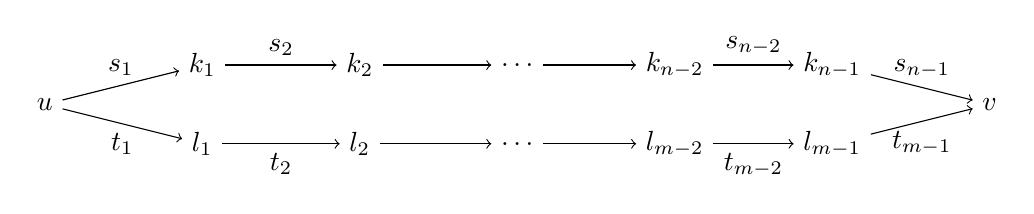
\begin{tikzpicture}
        \node (u) at (0,0) {\( u \)};
        \node (k1) at (2,0.5) {\( k_1 \)};
        \node (k2) at (4,0.5) {\( k_2 \)};
        \node (ketc) at (6,0.5) {\( \dots \)};
        \node (knm2) at (8,0.5) {\( k_{n-2} \)};
        \node (knm1) at (10,0.5) {\( k_{n-1} \)};
        \node (v) at (12,0) {\( v \)};
        \node (l1) at (2,-0.5) {\( l_1 \)};
        \node (l2) at (4,-0.5) {\( l_2 \)};
        \node (letc) at (6,-0.5) {\( \dots \)};
        \node (lnm2) at (8,-0.5) {\( l_{m-2} \)};
        \node (lnm1) at (10,-0.5) {\( l_{m-1} \)};
        \draw[->] (u) -- (k1) node [midway,above] {\( s_1 \)};
        \draw[->] (k1) -- (k2) node [midway,above] {\( s_2 \)};
        \draw[->] (k2) -- (ketc);
        \draw[->] (ketc) -- (knm2); 
        \draw[->] (knm2) -- (knm1) node[midway,above] {\( s_{n-2} \)}; 
        \draw[->] (knm1) -- (v) node[midway,above] {\( s_{n-1} \)}; 
        \draw[->] (u) -- (l1) node[midway,below] {\( t_1 \)};
        \draw[->] (l1) -- (l2) node[midway,below] {\( t_2 \)};
        \draw[->] (l2) -- (letc);
        \draw[->] (letc) -- (lnm2); 
        \draw[->] (lnm2) -- (lnm1) node[midway,below] {\( t_{m-2} \)}; 
        \draw[->] (lnm1) -- (v) node[midway,below] {\( t_{m-1} \)}; 
        \end{tikzpicture}
    }
    \end{center}
    \noindent
    the equality \( h(s_1) \mathop{\star} h(s_2) \mathop{\star} \dots  \mathop{\star} h(s_{n-1}) \mathop{=} h(t_1) \mathop{\star} h(t_2) \mathop{\star} \dots  \mathop{\star} h(t_{m-1}) \) holds.
\end{definition}

\begin{definition}[Pushout \cite{barr1990category}]
    \label{def:cat:po}
    \ \newline
\noindent
\begin{minipage}{0.7\textwidth}  
    A \textbf{pushout} of a span \( B \overset{\alpha}{\leftarrow} A \overset{\beta}{\rightarrow} C \), as shown on the right, is defined as a cospan \( B \overset{\beta'}{\rightarrow} D \overset{\alpha'}{\leftarrow} C \) such that \( \alpha \mathop{\star} \beta' \mathop{=} \beta \mathop{\star} \alpha' \), and for every cospan \( B \overset{\gamma'}{\rightarrow} E \overset{\gamma}{\leftarrow} C \), if \( \alpha \mathop{\star} \gamma' \mathop{=} \beta \mathop{\star} \gamma \) holds, then there exists a unique morphism \(\delta : D \mathop{\to} E\) such that \( \gamma' \mathop{=} \beta' \mathop{\star} \delta \) and \( \gamma \mathop{=} \alpha' \mathop{\star} \delta \).
\end{minipage}
\hfill
\begin{minipage}{0.299\textwidth}
    \hfill
\resizebox{0.9\textwidth}{!}{
           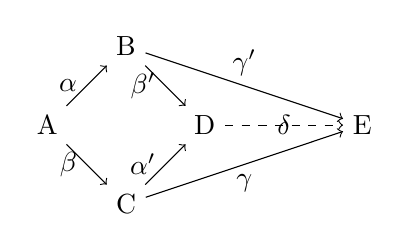
\begin{tikzpicture}
                \node (i) at (0,0) {A};
                \node (r) at (1,1) {B};
                \node (c) at (1,-1) {C};
                \node (h) at (2,0) {D};
                % \node () at (1,-1) {\( \Delta \)};
                \draw[->]  (i) -- (r) node [midway,left] {$ \alpha $};
                \draw[->] (c) -- (h) node [midway,left] {$ \alpha' $};
                \draw[->] (r) -- (h) node[midway, left] {$ \beta' $};
                \draw[->] (i) -- (c) node[midway, left] {$ \beta $};
                \node (d') at (4,0) {E};
                \draw[->] (c) -- (d') node [midway,below]{$ \gamma $};
                \draw[->] (r) -- (d') node [midway,above]{$ \gamma' $};
                \draw[->,dashed] (h) -- (d') node [midway]{$ \delta $};
            \end{tikzpicture}
}
\end{minipage}
The diagram involving \( (\alpha, \beta, \alpha', \beta') \) is called the \textbf{pushout square}, with \(D\) as the \textbf{pushout object}. The existence of a unique morphism is known as the universal mapping property of the pushout.
\end{definition} 
\begin{example}
    \label{ex:cat:po}
    Consider the square in \textbf{Graph} illustrated below.
    A pushout of the span \( B \overset{\alpha}{\leftarrowtail} A \overset{\beta}{\rightarrowtail} C \) is the cospan \( C \overset{\alpha'}{ 
    \rightarrowtail} D \overset{\beta'}{\leftarrowtail} B \), where pushout object \( D \) is the graph union of $B$ and $C$ and the morphisms \( \alpha' \) and \( \beta' \) are inclusion functions. 

    \begin{center} 
        \resizebox{0.45\textwidth}{!}{
        \begin{tikzpicture} 
            \graphbox{\( B \)}{40mm}{20mm}{34mm}{12mm}{2mm}{2mm}{
                \coordinate (o) at (0mm,-8mm); 
                \node[draw,circle] (l1) at ($(o)+(-10mm,0mm)$) {1};
                \node[draw,circle] (l2) at ($(l1)+(2,0)$) {2};
                \node[draw,circle,red] (l3) at ($(l1)+(1,0)$) {3};
                \draw[->,red] (l1) -- (l3) node[midway,above] {$a$};
                \draw[->,red] (l3) -- (l2) node[midway,above] {$a$};
            } 
    
            \graphbox{\( A \)}{0mm}{0mm}{34mm}{12mm}{2mm}{2mm}{
                \coordinate (o) at (0mm,-8mm); 
                \node[draw,circle] (l1) at ($(o)+(-10mm,0mm)$) {1};
                \node[draw,circle] (l2) at ($(l1)+(2,0)$) {2};
            }  
            \graphbox{\( D \)}{90mm}{5mm}{34mm}{22mm}{2mm}{-3mm}{
                \coordinate (o) at (0mm,-3mm); 
                \node[draw,circle] (l1) at ($(o)+(-10mm,0mm)$) {1};
                \node[draw,circle] (l2) at ($(l1)+(2,0)$) {2};
                \node[draw,circle,red] (l3) at ($(l1)+(1,0)$) {3};
                \node[draw,circle,blue] (l4) at ($(l2)+(0,-1)$) {6};
                \draw[->,red] (l1) -- (l3) node[midway,above] {$a$};
                \draw[->,red] (l3) -- (l2) node[midway,above] {$a$};
                \draw[->,blue] (l2) -- (l4) node[midway,right] {$a$};
                \node[draw,circle,blue] (l6) at ($(l1)+(0,-1)$) {7};
                \draw[<-,blue] (l1) -- (l6) node[midway,left] {$a$};
                \draw[->,blue] (l2) edge[out=-135,in=-45]node[midway,below] {$a$} (l1) ;
            }    
     
            \graphbox{\( C  \)}{40mm}{-20mm}{34mm}{22mm}{2mm}{-3mm}{
                \coordinate (o) at (0mm,-3mm); 
                \node[draw,circle] (l1) at ($(o)+(-10mm,0mm)$) {1};
                \node[draw,circle] (l2) at ($(l1)+(2,0)$) {2};
                \node[draw,circle,blue] (l4) at ($(l2)+(0,-1)$) {6};
                \draw[->,blue] (l2) -- (l4) node[midway,right] {$a$};
                \draw[->,blue] (l2) edge[out=-135,in=-45]node[midway,below] {$a$} (l1) ;
                \node[ draw,circle,blue] (l6) at ($(l1)+(0,-1)$) {7};
                \draw[<-,blue] (l1) -- (l6) node[midway,left] {$a$};
            }      
            % K to L
            \draw[>->] (17mm,5mm) -- node[above] {$\alpha$} (37mm,15mm);
            % C to G
            \draw[>->] (76mm,-28mm)-- node[below] {$\alpha'$} (104mm,-20mm) ;
            % K to C
            \draw[>->] (17mm,-17mm) -- node[below] {$\beta$} (37mm,-28mm);
            % L to G
            \draw[>->] (76mm,16mm) -- node[above] {$\beta'$} (104mm,7mm);
            \node () at (57mm,-6mm) {$PO$};
        \end{tikzpicture}
        }
    \end{center}
\end{example}
\begin{definition}[Pullback \cite{pierce1991basic}]
    \label{def:cat:pb}
    \ \newline
\noindent
\begin{minipage}{0.7\textwidth}  
   A \textbf{pullback} of a cospan \(B \overset{\beta'}{\rightarrow} D \overset{\alpha'}{\leftarrow} C \), as shown on the right, is defined as a span \( B \overset{\alpha}{\leftarrow} A \overset{\beta}{\rightarrow} C \) such that \( \alpha \mathop{\star} \beta' \mathop{=} \beta \mathop{\star} \alpha' \), and for every span \( B \overset{\gamma'}{\leftarrow} E \overset{\gamma}{\rightarrow} C \) if \(\gamma' \mathop{\star} \beta' \mathop{=} \gamma \mathop{\star} \alpha'\) holds, then there exists a unique morphism \(\delta: E \mathop{\to} A\) such that $\gamma' \mathop{=} \delta \mathop{\star} \alpha$ and $\gamma \mathop{=} \delta \mathop{\star} \beta$. 
\end{minipage}
\hfill
\begin{minipage}{0.299\textwidth}
    \hfill
\resizebox{0.9\textwidth}{!}{
            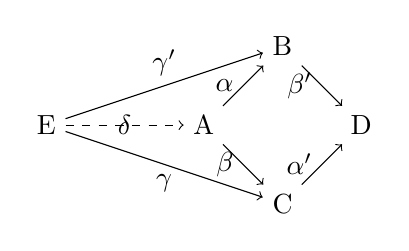
\begin{tikzpicture}
                \node (i) at (0,0) {A};
                \node (r) at (1,1) {B};
                \node (c) at (1,-1) {C};
                \node (h) at (2,0) {D};
                % \node () at (1,-1) {\( \Delta \)};
                \draw[->]  (i) -- (r) node [midway,left] {$\alpha$};
                \draw[->] (c) -- (h) node [midway,left] {$\alpha'$};
                \draw[->] (r) -- (h) node[midway, left] {$\beta'$};
                \draw[->] (i) -- (c) node[midway, left] {$\beta$};
                \node (d') at (-2,0) {E};
                \draw[<-] (c) -- (d') node [midway,below]{$\gamma$};
                \draw[<-] (r) -- (d') node [midway,above]{$\gamma'$};
                \draw[->, dashed] (d') -- (i) node [midway]{$\delta$};
            \end{tikzpicture}
}
\end{minipage}
The diagram involving \( (\alpha, \beta, \alpha', \beta') \) is called the \textbf{pullback square}, with \(A\) as the \textbf{pullback object}. The existence of a unique morphism is known as the universal mapping property of the pullback.
\end{definition} 
 
\begin{definition}
    \label{def:cat:pb}
    Consider the square in Example~\ref{ex:cat:po}. A pullback of the cospan \( C \overset{\alpha'}{\rightarrowtail} D \overset{\beta'}{\leftarrowtail} B \) is the span \( B \overset{\alpha}{\leftarrowtail} A \overset{\beta}{\rightarrowtail} C \), where pullback object \( A \) is the graph intersection of $B$ and $C$ and the morphisms \( \alpha \) and \( \beta \) are inclusion functions.
\end{definition}
\begin{notation}
    When the context makes it clear, a morphism \( h : A \mathop{\to} B \) will be denoted by \( h_{AB} \), and diagrams will be referred to by their nodes, as is standard in geometry. For example, the diagram involving morphisms \( ( \alpha, \beta, \alpha', \beta' ) \) in Definition~\ref{def:cat:po} will be denoted by \( ACDB \) or \( ABDC \).
\end{notation}   
    
    \section{Graph Rewriting Systems (GRS)} 
    
    \subsection{DPO GRS}
    \begin{definition}[Rewriting rule, Match~\cite{ehrig1997algebraic}]
        \label{def:grs:dpo_rule}
      A \textbf{DPO rewriting rule} $\rho$ is a span \( L \overset{l}{\leftarrow} K \overset{r}{\rightarrow} R \), where \( K \) is the \textbf{interface}, \( L \) is the \textbf{left-hand-side graph}, denoted \( \operatorname{lhs}(\rho) \), and \( R \) is the \textbf{right-hand-side graph}, denoted \( \operatorname{rhs}(\rho) \). The rule is \textbf{left-monic} if the morphism \( l \) is monic, \textbf{right-monic} if the morphism \( r \) is monic, \textbf{monic} if it is left- and right-monic \todo{Do you consider rules where this is not the case?}  
      A \textbf{match} of the rule in an graph \( G \) is a morphism \( m: L \mathop{\rightarrow} G \).   
      \end{definition}
    
      \begin{example}
        \label{ex:grsaa}
        The injective DPO rule from \cite[Example 6]{bruggink2014termination} will be used as a running example throughout this paper to illustrate the concepts disccussed.
        \begin{center} 
            \resizebox{0.7\textwidth}{!}{
            \begin{tikzpicture}
                \graphbox{$L$}{0mm}{0mm}{34mm}{15mm}{2mm}{-5mm}{
                    \coordinate (o) at (0mm,-3mm); 
                    \node[draw,circle] (l1) at ($(o)+(-10mm,0mm)$) {1};
                    \node[draw,circle] (l2) at ($(l1)+(2,0)$) {2};
                    \node[draw,circle] (l3) at ($(l1)+(1,0)$) {3};
                    \draw[->] (l1) -- (l3) node[midway,above] {$a$};
                    \draw[->] (l3) -- (l2) node[midway,above] {$a$};
                }     
                \graphbox{$K$}{40mm}{0mm}{24mm}{15mm}{2mm}{-5mm}{
                    \coordinate (o) at (5mm,-3mm); 
                    \node[draw,circle] (l1) at ($(o)+(-10mm,0mm)$) {1};
                    \node[draw,circle] (l2) at ($(l1)+(1,0)$) {2};
                    % \node[draw,circle] (l3) at ($(l1)+(1,0)$) {$\ $};
                    % \draw[->] (l1) -- (l3) node[midway,above] {$a$};
                    % \draw[->] (l3) -- (l2) node[midway,above] {$a$};
                }    
                \graphbox{$R$}{70mm}{0mm}{45mm}{15mm}{2mm}{-5mm}{
                    \coordinate (o) at (-5mm,-3mm); 
                    \node[draw,circle] (l1) at ($(o)+(-10mm,0mm)$) {1};
                    \node[draw,circle] (l2) at ($(l1)+(3,0)$) {2};
                    \node[draw,circle] (l3) at ($(l1)+(1,0)$) {4};
                    \node[draw,circle] (l4) at ($(l1)+(2,0)$) {5};
                    \draw[->] (l1) -- (l3) node[midway,above] {$a$};
                    \draw[->] (l3) -- (l4) node[midway,above] {$b$};
                    \draw[->] (l4) -- (l2) node[midway,above] {$a$};
                }    
                \node () at (37mm,-8mm) {$\leftarrowtail$};
                \node () at (67mm,-8mm) {$\rightarrowtail$};
                % \draw[>->] (51mm,2mm) -- (52mm,3mm);
            \end{tikzpicture}
            }
        \end{center}
      \end{example}
      
      \begin{definition}[Witness, Rewriting step \cite{endrullis2024generalized}]
        \label{def:rewriting_step}
          \ \newline
          \noindent
          \begin{minipage}{0.72\textwidth}
            A DPO diagram $\delta$ is a diagram as shown on the right.
            This diagram $\delta$ is a \textbf{witness} for the \textbf{rewriting step} from \( G \) to \( H \) using the rule \( \rho \) and match \( m \), denoted \( G \mathop{\Rightarrow}_\rho^m H \) or \( G \mathop{\Rightarrow}_\rho^\delta H \). We denote $\operatorname{left}(\delta)$ and $\operatorname{right}(\delta)$ the pushout squares $KLGC$ and $KRHC$, respectively.
          \end{minipage}
          \hfill
          \begin{minipage}{0.28\textwidth}
                % \begin{center}
                \hfill
                \resizebox{\textwidth}{!}{
                \begin{tikzpicture}
                  % [node distance=11mm]
                  \node (I) {$K$};
                  \node (L) [left of=I] {$L$};
                  \node (R) [right of=I] {$R$};
                  \node (G) [below of=L] {$G$};
                  \node (C) [below of=I] {$C$};
                  \node (H) [below of=R] {$H$};
                  \draw [->] (I) to  node [midway,above] {$l$} (L);
                  \draw [->] (I) to  node [midway,above] {$r$} (R);
                  \draw [->] (L) to node [midway,left] {$m$} (G);
                  \draw [->] (I) to (C);
                  \draw [->] (R) to node [midway,right] {$m'$} (H);
                  \draw [->] (C) to node [midway,below] {$l'$} (G);
                  \draw [->] (C) to node [midway,below] {$r'$} (H);
                  \node [at=($(I)!.5!(G)$)] {\normalfont PO};
                  \node [at=($(I)!.5!(H)$)] {\normalfont PO};
                \end{tikzpicture}
              % \end{center}
              }
              \end{minipage}
        \end{definition}
    
        \begin{example}
            \label{ex:rewriting_step_grs_aa}
            The DPO diagram below defines a rewriting step using the rule from Example~\ref{ex:grsaa}.
            \begin{center} 
                \resizebox{0.7\textwidth}{!}{
                \begin{tikzpicture}
                    \graphbox{\( L \)}{0mm}{-3mm}{34mm}{12mm}{2mm}{2mm}{
                        \coordinate (o) at (0mm,-8mm); 
                        \node[draw,circle] (l1) at ($(o)+(-10mm,0mm)$) {1};
                        \node[draw,circle] (l2) at ($(l1)+(2,0)$) {2};
                        \node[draw,circle] (l3) at ($(l1)+(1,0)$) {3};
                        \draw[->] (l1) -- (l3) node[midway,above] {$a$};
                        \draw[->] (l3) -- (l2) node[midway,above] {$a$};
                    } 
            
                    \graphbox{\( K \)}{40mm}{-3mm}{34mm}{12mm}{2mm}{2mm}{
                        \coordinate (o) at (0mm,-8mm); 
                        \node[draw,circle] (l1) at ($(o)+(-10mm,0mm)$) {1};
                        \node[draw,circle] (l2) at ($(l1)+(2,0)$) {2};
                    }  
            
                    \graphbox{\( R \)}{80mm}{-3mm}{45mm}{12mm}{2mm}{2mm}{
                        \coordinate (o) at (-5mm,-8mm); 
                        \node[draw,circle] (l1) at ($(o)+(-10mm,0mm)$) {1};
                        \node[draw,circle] (l2) at ($(l1)+(3,0)$) {2};
                        \node[draw,circle] (l3) at ($(l1)+(1,0)$) {4};
                        \node[draw,circle] (l4) at ($(l1)+(2,0)$) {5};
                        \draw[->] (l1) -- (l3) node[midway,above] {$a$};
                        \draw[->] (l3) -- (l4) node[midway,above] {$b$};
                        \draw[->] (l4) -- (l2) node[midway,above] {$a$};
                    }    
            
                    \graphbox{\( G \)}{0mm}{-22mm}{34mm}{22mm}{2mm}{-3mm}{
                        \coordinate (o) at (0mm,-3mm); 
                        \node[draw,circle] (l1) at ($(o)+(-10mm,0mm)$) {1};
                        \node[draw,circle] (l2) at ($(l1)+(2,0)$) {2};
                        \node[draw,circle] (l3) at ($(l1)+(1,0)$) {3};
                        \node[draw,circle] (l4) at ($(l2)+(0,-1)$) {6};
                        \draw[->] (l1) -- (l3) node[midway,above] {$a$};
                        \draw[->] (l3) -- (l2) node[midway,above] {$a$};
                        \draw[->] (l2) -- (l4) node[midway,right] {$a$};
                        \node[draw,circle] (l6) at ($(l1)+(0,-1)$) {7};
                        \draw[<-] (l1) -- (l6) node[midway,left] {$a$};
                        \draw[->] (l2) edge[out=-135,in=-45]node[midway,below] {$a$} (l1) ;
                    }    
            
                    \graphbox{\( C  \)}{40mm}{-22mm}{34mm}{22mm}{2mm}{-3mm}{
                        \coordinate (o) at (0mm,-3mm); 
                        \node[draw,circle] (l1) at ($(o)+(-10mm,0mm)$) {1};
                        \node[draw,circle] (l2) at ($(l1)+(2,0)$) {2};
                        \node[draw,circle] (l4) at ($(l2)+(0,-1)$) {6};
                        \draw[->] (l2) -- (l4) node[midway,right] {$a$};
                        \draw[->] (l2) edge[out=-135,in=-45]node[midway,below] {$a$} (l1) ;
                        \node[ draw,circle] (l6) at ($(l1)+(0,-1)$) {7};
                        \draw[<-] (l1) -- (l6) node[midway,left] {$a$};
                    }    
            
                    \graphbox{\( H \)}{80mm}{-22mm}{45mm}{22mm}{2mm}{-3mm}{
                        \coordinate (o) at (-5mm,-3mm); 
                        \node[draw,circle] (l1) at ($(o)+(-10mm,0mm)$) {1};
                        \node[draw,circle] (l2) at ($(l1)+(3,0)$) {2};
                        \node[draw,circle] (l3) at ($(l1)+(1,0)$) {4};
                        \node[draw,circle] (l4) at ($(l1)+(2,0)$) {5};
                        \node[ draw,circle] (l5) at ($(l2)+(0,-1)$) {6};
                        \node[ draw,circle] (l6) at ($(l1)+(0,-1)$) {7};
                        \draw[<-] (l1) -- (l6) node[midway,left] {$a$};
                        \draw[->] (l1) -- (l3) node[midway,above] {$a$};
                        \draw[->] (l3) -- (l4) node[midway,above] {$b$};
                        \draw[->] (l4) -- (l2) node[midway,above] {$a$};
                        \draw[->] (l2) -- (l5) node[midway,right] {$a$};
                        \draw[->] (l2) edge[out=-135,in=-45]node[midway,below] {$a$} (l1) ;
                    }    
            
                    \node () at (37mm,-8mm) {\( \leftarrowtail \)}; % K -> L
                    \node () at (77mm,-8mm) {\( \rightarrowtail \)}; % K -> R
                    \node () at (15mm,-18mm) {\( m\ \downarrowtail \)};
                    \node () at (37mm,-33mm) {\( \leftarrowtail \)};
                    \node () at (58mm,-18mm) {\( \downarrowtail \)};
                    \node () at (102mm,-18mm) {\( \downarrowtail \)};
                    \node () at (77mm,-33mm) {\( \rightarrowtail \)}; % C -> H
                \end{tikzpicture}
                }
            \end{center}
          \end{example}
    
    \begin{definition}[Rewriting framework \cite{endrullis2024generalized}]
        A \textbf{DPO rewriting framework} $\mathfrak{F}$ is a mapping of DPO rewriting rules to classes of DPO diagrams such that, for every rule $\rho$, $\mathfrak{F}(\rho)$ is a class of DPO diagrams with top-span $\rho$.
      \end{definition}
    
    \trackedtext{
      \begin{definition}[Rewriting relation]
        The \textbf{rewriting relation $\mathop{\Rightarrow}_{\mathfrak{dpo},\mathfrak{F},\rho}$ induced by a rule $\rho$ in $\mathfrak{F}$} is defined as follows: $G \mathop{\Rightarrow}_{\mathfrak{dpo},\mathfrak{F},\rho} H$ iff $G \mathop{\Rightarrow}_\rho^\delta H$ for some $\delta \mathop{\in} \mathfrak{F}(\rho)$. 
          % for some $\delta \mathop{\in} \mathfrak{F}(\rho)$
          The \textbf{DPO rewriting relation $\mathop{\Rightarrow}_{\mathcal{R},\mathfrak{F}}$ induced by a set $\mathcal{R}$ of DPO rewriting rules in $\mathfrak{F}$} is given by: $G \mathop{\Rightarrow}_{\mathfrak{dpo}, \mathfrak{F},\mathcal{R}} H$ iff $G \mathop{\Rightarrow}_{\mathfrak{dpo},\mathfrak{F}, \rho} H$ for some $\rho \mathop{\in} \mathcal{R}$. When $\mathfrak{F}$ is clear from the context, we 
          suppress $\mathfrak{F}$ and 
          write $\mathop{\Rightarrow}_{\mathfrak{dpo},\rho}$ and $\mathop{\Rightarrow}_{\mathfrak{dpo},\mathcal{R}}$.
      \end{definition} 
    }

    \begin{definition}[DPO Graph Rewriting System]
      Let $M, \mathfrak{M}, W, \mathfrak{W}, \mathfrak{I}$ be the class of DPO matches, the match mechanism, the class of DPO witnesses, the witness mechanism and the interpretation function, respectively, defined in Definition~\ref{def:grs:dpo_rule}.
      Let $\mathfrak{F}$ be a DPO rewriting framework as defined in Definition~\ref{def:rewriting_framework}.
      The rewriting system $(\mathbf{Graph}, \mathcal{R}, M, \mathfrak{M}, W, \mathfrak{W}, \mathfrak{I}, \mathfrak{F})$ is called a \textbf{DPO Graph Rewriting System in $\mathfrak{F}$}.
    \end{definition}


    \color{red}    
    
    
    dpo
    dpo limitations ;
    les autres differences
    
    \begin{proposition}[to do]
        inclusion : dpo $>$ spo $>$ ...
    \end{proposition}
    
    \begin{itemize}
        \item we are only able to delete nodes if they do not leave any edges “dangling” (called the gluing condition),This can be considered a pleasant safety feature, but also a limitation. However, since GLS never delete or duplicate nodes, DPO GRS is a well studied approach with advanced termination method.
        \item the most dominant graph rewriting method, called the Double Pushout (DPO) approach, combines the pushout complement approach (with the injectivity requirement on $\rho$) with the ToyPO approach. In doing so, it enables the specification of rewrite steps with deletion, identification and addition features, for matches m that satisfy the gluing condition.
        \item Alternatives to the DPO approach avoid the construction of pushout complements. For instance, the Single Pushout (SPO) approach [17] relies on a single pushout construction, but uses partial graph homomorphisms instead of total morphisms, in order to specify deletion. In this approach, the gluing condition no longer needs to be checked either: all edges incident to a removed vertex are simply deleted.
        \item As another example, the Sesqui-Pushout (corradini2006sesqui) approach [8] replaces the first PO square of DPO by what is called a final pullback complement square. This square allows duplication with deterministic behavior, and like SPO, deletes any edges that would be left dangling.
        \item !!! implicite deletion of nodes or edges is a problem when we want to prove the termination 
        \item[handbook] 
            As shown for example in [2], in category Graph, the pushout complement object of two morphisms <b,g> exsits iff the gluing condition is satisfied; moreover, it is unique if b is injective.
            \begin{proposition}[Existence of Pushout Complements]
                Let $b : A \mathop{\to} B$ and $g : B \mathop{\to} D$ be two morphisms in $\mathbf{Graph}$. Then there exists a pushout complement $\langle C, c : A \mathop{\to} C, f : C \mathop{\to} D \rangle$ of $\langle b, g \rangle$ if and only if the following conditions are satisfied:
                
                \begin{itemize}
                    \item \textbf{[Dangling condition]} No edge $e \mathop{\in} D_E - g_E(B_E)$ is incident to any node in $g_V(B_V - b_V(A_V))$.
                    \item \textbf{[Identification condition]} There is no $x, y \mathop{\in} B_V \mathop{\cup} B_E$ such that $x \mathop{\neq} y$, $g(x) \mathop{=} g(y)$ and $y \notin b(A_V \mathop{\cup} A_E)$.
                \end{itemize}
                
                In this case, we say that $\langle b, g \rangle$ satisfies the \textit{gluing condition} (or $g$ satisfies the gluing condition with respect to $b$). If moreover morphism $b$ is injective, then the pushout complement is unique up to isomorphism, i.e., if $\langle C, c, f \rangle$ and $\langle C', c', f' \rangle$ are two pushout complements of $\langle b, g \rangle$, then there is an isomorphism $\varphi : C \mathop{\to} C'$ such that $\varphi \circ c \mathop{=} c'$ and $f' \circ \varphi \mathop{=} f$.
                \end{proposition}
            
        \item[adhesive categories] In D-p rewriting, a rewrite rule is given as a span 
        \begin{tikzcd}
            L & K \arrow[l] \arrow[r] & R
        \end{tikzcd}. 
        Roughly, The intuition is that \( L \) forms the left-hand side of the rewrite rule, \( R \) forms the right-hand side and \( K \), common to both \( L \) and \( R \), is the sub-structure to be unchanged as the rule is applied. To apply the rule to a structure \( C \), one first needs to find a match \( L \mathop{\to} C \) of \( L \) within \( C \). The rule is then applied by constructing the missing parts (\( E, D \) and arrows) of the following diagram
        \begin{figure}[H]
            \begin{tikzcd}
                L \arrow[d]&  K \arrow[d] \arrow[l] \arrow[r] & R  \arrow[d]\\
                C  & E \arrow[l]  \arrow[r] & D
            \end{tikzcd} 
        \end{figure}
        in a way which ensures that the two squares are pushout diagrams. Once such a diagram is constructed we may deduce that \( C \mathop{\Rightarrow} D \), that is, \( C \) rewrites to \( D \).
        
    \end{itemize}
    
    
    
    \begin{definition}[DPO Graph Rewriting System \cite{endrullis2024generalized}]
        A \textbf{DPO Graph Rewriting System} is a DPO rewriting system on $\mathbf{Graph}$.  
    \end{definition}
    
    When a direct graph transformation with a production p and a match m is performed, all the vertices and edges which are matched by$ L \mathop{\setminus} K$ are removed from G. The removed part is not a graph, in general, but the remaining structure $D := (G \mathop{\setminus} m(L)) \mathop{\cup}  m(K)$ still has to be a graph. This means that the match $m$ has to satisfy a suitable gluing condition, which makes sure that the gluing of $L\mathop{\setminus} K$ and $D$ is equal to G. In the second step of a graph rewriting step, the graph $D$ is glued together with $R \mathop{\setminus} K$ to obtain the derived graph $H$ . For gluing newly created vertices and edges into D,the graph $m(K)$ and $r(K)$ are used: nodes and edges with the same pre-image will be unified.
    
    Trees form a sub-category of $\mathbf{Graph}$, denoted as $\mathbf{Tree}$.
    \begin{definition}[DPO Tree Rewriting System]
       A \textbf{DPO Tree Rewriting System} is a DPO rewriting system on $\mathbf{Tree}$.
    \end{definition}
    
    todo : Def functor F
    \begin{proposition} 
       The functor $F: \mathbf{Tree} \mathop{\to} \mathbf{Trs}$ is isomorphic.
    \end{proposition}
    todo : def functor F
    \begin{proposition}
       
       $F$ is a functor from the category of GLS to the category of linear DPO graph rewriting.
    \end{proposition}
    
    \begin{remark}
       a GLS is essentially a DPO GRS. Its simplicity compare with respect to DPO GRS is that, in the definition of rewriting step,it replaces the DPO diagram by "the underlying graph does not change", and deletion add addition of labeled arrows by the relabeling of unlabeled arrows. Its semantic is more intuitive but there is a price to pay compare to DPO GRS: we need to constantly renaming nodes. 
    \end{remark}
    
    \begin{remark}
      A TRS is essentially a DPO Tree rewriting system, which replace the DPO diagram in the definition of rewriting stemp by choosing the root node of lhs and rhs terms as interface (which is a very intuitive choice). A part hitorical, there is no reason to prefer TRS to DPO Tree rewriting.
    \end{remark}
    \color{black} 
    
    \subsection{DPO GRS with Negative Application Condition}
    \begin{definition}[Rewriting rule, Match~\cite{bottoni2010atermination}]
        \label{def:grs:dpo_nac_rule}
        A \textbf{DPO rewriting rule with a negative application condition} $\varphi$ is an ordered pair \( \left( n , \rho \right) \) where $n$ is a monomorphism and $\rho$ is an monic DPO rewriting rule
         such that $\operatorname{codom}(\operatorname{lhs}(\rho)) \mathop{=} \operatorname{dom}(n)$.
         
         A rule is denoted \( N \overset{n}{\leftarrowtail} L \overset{l}{\leftarrowtail} K \overset{r}{\rightarrowtail} R \) with $\rho \mathop{=} (L \overset{l}{\leftarrowtail} K \overset{r}{\rightarrowtail} R) $.
    
        A match of the rule in an object \( G \) is a monomorphism \( m: L \mathop{\rightarrow} G \) such that there is no monomorphism \( q: N \mathop{\rightarrow} G \) such that \( n \mathop{\star} q \mathop{=} m \), as illustrated below.
    
        A DPO diagram as shown below is a \textbf{witness} for a \textbf{rewriting step} from \( G \) to \( H \) using the rule $\varphi$ and match \( m \), denoted \( G \mathop{\Rightarrow}_\rho^m H \) or \( G \mathop{\Rightarrow}_\rho^\delta H \). 
        % We denote $\operatorname{left}(\delta)$ and $\operatorname{right}(\delta)$ the pushout squares $KLGC$ and $KRHC$, respectively.
    
    \begin{figure}[H]
        \begin{tikzpicture} 
            % Define nodes
            \node (K)  {K};
            \node (L) [left=of K] {L};
            \node (R) [right=of K] {R};
            \node (N) [left=of L] {N};
            \node (G) [below=of L] {G};
            \node (D) [below=of K] {D};
            \node (H) [below=of R] {H};
    
            % Draw arrows
            % Top row
            \draw[>->] (L) -- node[above] {n} (N);
            \draw[>->] (K) -- node[above] {$l$} (L);
            \draw[>->] (K) -- node[above] {$r$} (R);
          
            % Vertical arrows
            \draw[>->] (L) -- node[left] {$m$} (G);
            \draw[>->] (K) --  (D);
            \draw[>->] (R) --  (H);
          
            % Bottom row
            \draw[>->] (G) --  (D);
            \draw[>->] (D) --   (H);
          
            % Bent arrow from G to N
            \draw[>->, bend right,red,dashed] (N) to node[below] {q} (G);
    
            \node at ($(N)!0.5!(G)$) {\textcolor{red}{$\mathop{\neq}$}};
            \node at ($(K)!0.5!(G)$) {$\mathrm{PO}$};
            \node at ($(K)!0.5!(H)$) {$\mathrm{PO}$};
          \end{tikzpicture}
          \label{fig:grs:dpo_nac_rule}
    \end{figure}
    \end{definition}
    \begin{example}
      The following diagram illustrates a DPO rewriting rule with a negative application condition:
      \begin{center} 
        \resizebox{0.7\textwidth}{!}{
        \begin{tikzpicture}
          \graphbox{$N$}{-40mm}{0mm}{34mm}{20mm}{2mm}{-5mm}{
            \coordinate (o) at (0mm,-3mm); 
            \node[draw,circle] (l1) at ($(o)+(-10mm,0mm)$) {1};
            \node[draw,circle] (l2) at ($(l1)+(2,0)$) {2};
            \node[draw,circle] (l3) at ($(l1)+(1,0)$) {3};
            \draw[->] (l1) -- (l3) node[midway,above] {$a$};
            \draw[->] (l3) -- (l2) node[midway,above] {$a$};
            \draw[->] (l2) edge[out=-135,in=-45]node[midway,below] {$a$} (l1) ;
        }  
            \graphbox{$L$}{0mm}{0mm}{34mm}{15mm}{2mm}{-5mm}{
                \coordinate (o) at (0mm,-3mm); 
                \node[draw,circle] (l1) at ($(o)+(-10mm,0mm)$) {1};
                \node[draw,circle] (l2) at ($(l1)+(2,0)$) {2};
                \node[draw,circle] (l3) at ($(l1)+(1,0)$) {3};
                \draw[->] (l1) -- (l3) node[midway,above] {$a$};
                \draw[->] (l3) -- (l2) node[midway,above] {$a$};
            }     
            \graphbox{$K$}{40mm}{0mm}{24mm}{15mm}{2mm}{-5mm}{
                \coordinate (o) at (5mm,-3mm); 
                \node[draw,circle] (l1) at ($(o)+(-10mm,0mm)$) {1};
                \node[draw,circle] (l2) at ($(l1)+(1,0)$) {2};
                % \node[draw,circle] (l3) at ($(l1)+(1,0)$) {$\ $};
                % \draw[->] (l1) -- (l3) node[midway,above] {$a$};
                % \draw[->] (l3) -- (l2) node[midway,above] {$a$};
            }    
            \graphbox{$R$}{70mm}{0mm}{45mm}{15mm}{2mm}{-5mm}{
                \coordinate (o) at (-5mm,-3mm); 
                \node[draw,circle] (l1) at ($(o)+(-10mm,0mm)$) {1};
                \node[draw,circle] (l2) at ($(l1)+(3,0)$) {2};
                \node[draw,circle] (l3) at ($(l1)+(1,0)$) {4};
                \node[draw,circle] (l4) at ($(l1)+(2,0)$) {5};
                \draw[->] (l1) -- (l3) node[midway,above] {$a$};
                \draw[->] (l3) -- (l4) node[midway,above] {$b$};
                \draw[->] (l4) -- (l2) node[midway,above] {$a$};
            }    
            \node () at (-3mm,-8mm) {$\leftarrowtail$};
            \node () at (37mm,-8mm) {$\leftarrowtail$};
            \node () at (67mm,-8mm) {$\rightarrowtail$};
            % \draw[>->] (51mm,2mm) -- (52mm,3mm);
        \end{tikzpicture}
        }
    \end{center}
      The rewriting step in Example~\ref{ex:rewriting_step_grs_aa} is not possible with this rule in DPO rewriting with negative application conditions, because there exists a monomorphism \( q: N \mathop{\rightarrow} G \) such that \( n \mathop{\star} q \mathop{=} m \) as shown in the diagram below.
      \begin{center} 
        \resizebox{0.7\textwidth}{!}{
        \begin{tikzpicture}
          \graphbox{$N$}{-40mm}{0mm}{34mm}{20mm}{2mm}{-5mm}{
            \coordinate (o) at (0mm,-3mm); 
            \node[draw,circle] (l1) at ($(o)+(-10mm,0mm)$) {1};
            \node[draw,circle] (l2) at ($(l1)+(2,0)$) {2};
            \node[draw,circle] (l3) at ($(l1)+(1,0)$) {3};
            \draw[->] (l1) -- (l3) node[midway,above] {$a$};
            \draw[->] (l3) -- (l2) node[midway,above] {$a$};
            \draw[->] (l2) edge[out=-135,in=-45]node[midway,below] {$a$} (l1) ;
        }  
            \graphbox{\( L \)}{0mm}{-3mm}{34mm}{12mm}{2mm}{2mm}{
                \coordinate (o) at (0mm,-8mm); 
                \node[draw,circle] (l1) at ($(o)+(-10mm,0mm)$) {1};
                \node[draw,circle] (l2) at ($(l1)+(2,0)$) {2};
                \node[draw,circle] (l3) at ($(l1)+(1,0)$) {3};
                \draw[->] (l1) -- (l3) node[midway,above] {$a$};
                \draw[->] (l3) -- (l2) node[midway,above] {$a$};
            } 
    
            \graphbox{\( K \)}{40mm}{-3mm}{34mm}{12mm}{2mm}{2mm}{
                \coordinate (o) at (0mm,-8mm); 
                \node[draw,circle] (l1) at ($(o)+(-10mm,0mm)$) {1};
                \node[draw,circle] (l2) at ($(l1)+(2,0)$) {2};
            }  
    
            \graphbox{\( R \)}{80mm}{-3mm}{45mm}{12mm}{2mm}{2mm}{
                \coordinate (o) at (-5mm,-8mm); 
                \node[draw,circle] (l1) at ($(o)+(-10mm,0mm)$) {1};
                \node[draw,circle] (l2) at ($(l1)+(3,0)$) {2};
                \node[draw,circle] (l3) at ($(l1)+(1,0)$) {4};
                \node[draw,circle] (l4) at ($(l1)+(2,0)$) {5};
                \draw[->] (l1) -- (l3) node[midway,above] {$a$};
                \draw[->] (l3) -- (l4) node[midway,above] {$b$};
                \draw[->] (l4) -- (l2) node[midway,above] {$a$};
            }    
    
            \graphbox{\( G \)}{0mm}{-22mm}{34mm}{22mm}{2mm}{-3mm}{
                \coordinate (o) at (0mm,-3mm); 
                \node[draw,circle] (l1) at ($(o)+(-10mm,0mm)$) {1};
                \node[draw,circle] (l2) at ($(l1)+(2,0)$) {2};
                \node[draw,circle] (l3) at ($(l1)+(1,0)$) {3};
                \node[draw,circle] (l4) at ($(l2)+(0,-1)$) {6};
                \draw[->] (l1) -- (l3) node[midway,above] {$a$};
                \draw[->] (l3) -- (l2) node[midway,above] {$a$};
                \draw[->] (l2) -- (l4) node[midway,right] {$a$};
                \node[draw,circle] (l6) at ($(l1)+(0,-1)$) {7};
                \draw[<-] (l1) -- (l6) node[midway,left] {$a$};
                \draw[->] (l2) edge[out=-135,in=-45]node[midway,below] {$a$} (l1) ;
            }    
    
            \graphbox{\( C  \)}{40mm}{-22mm}{34mm}{22mm}{2mm}{-3mm}{
                \coordinate (o) at (0mm,-3mm); 
                \node[draw,circle] (l1) at ($(o)+(-10mm,0mm)$) {1};
                \node[draw,circle] (l2) at ($(l1)+(2,0)$) {2};
                \node[draw,circle] (l4) at ($(l2)+(0,-1)$) {6};
                \draw[->] (l2) -- (l4) node[midway,right] {$a$};
                \draw[->] (l2) edge[out=-135,in=-45]node[midway,below] {$a$} (l1) ;
                \node[ draw,circle] (l6) at ($(l1)+(0,-1)$) {7};
                \draw[<-] (l1) -- (l6) node[midway,left] {$a$};
            }    
    
            \graphbox{\( H \)}{80mm}{-22mm}{45mm}{22mm}{2mm}{-3mm}{
                \coordinate (o) at (-5mm,-3mm); 
                \node[draw,circle] (l1) at ($(o)+(-10mm,0mm)$) {1};
                \node[draw,circle] (l2) at ($(l1)+(3,0)$) {2};
                \node[draw,circle] (l3) at ($(l1)+(1,0)$) {4};
                \node[draw,circle] (l4) at ($(l1)+(2,0)$) {5};
                \node[ draw,circle] (l5) at ($(l2)+(0,-1)$) {6};
                \node[ draw,circle] (l6) at ($(l1)+(0,-1)$) {7};
                \draw[<-] (l1) -- (l6) node[midway,left] {$a$};
                \draw[->] (l1) -- (l3) node[midway,above] {$a$};
                \draw[->] (l3) -- (l4) node[midway,above] {$b$};
                \draw[->] (l4) -- (l2) node[midway,above] {$a$};
                \draw[->] (l2) -- (l5) node[midway,right] {$a$};
                \draw[->] (l2) edge[out=-135,in=-45]node[midway,below] {$a$} (l1) ;
            }    
            \draw[>->, bend right] (-21mm,-22mm) to node[below] {q} (-4mm,-33mm);
            \node () at (-3mm,-8mm) {$\leftarrowtail$};
            \node () at (37mm,-8mm) {\( \leftarrowtail \)}; % K -> L
            \node () at (77mm,-8mm) {\( \rightarrowtail \)}; % K -> R
            \node () at (15mm,-18mm) {\( m\ \downarrowtail \)};
            \node () at (37mm,-33mm) {\( \leftarrowtail \)};
            \node () at (58mm,-18mm) {\( \downarrowtail \)};
            \node () at (102mm,-18mm) {\( \downarrowtail \)};
            \node () at (77mm,-33mm) {\( \rightarrowtail \)}; % C -> H
        \end{tikzpicture}
        }
    \end{center}
    \end{example}
    
    \begin{definition}[Rewriting framework]
      \label{def:dponac:rewriting_framework}
      A framework of rewriting with a negative application condition $\mathfrak{F}$ is a mapping of DPO rewriting rules with a negative condition to classes of diagrams as illustrated in Definition~\ref{def:grs:dpo_nac_rule} such that, for every rule $\varphi =(n, \rho)$, every diagram in $\mathfrak{F}(\varphi)$ has $\rho$ as the top-span of the DPO subdiagram.
    \end{definition}

    \trackedtext{
      \begin{definition}[Rewriting relation]
        The \textbf{rewriting relation $\mathop{\Rightarrow}_{\mathfrak{dponac},\mathfrak{F},\rho}$ induced by a rule $\rho$ in $\mathfrak{F}$} is defined as follows: $G \mathop{\Rightarrow}_{\mathfrak{dponac},\mathfrak{F},\rho} H$ iff $G \mathop{\Rightarrow}_\rho^\delta H$ for some $\delta \mathop{\in} \mathfrak{F}(\rho)$. 
          % for some $\delta \mathop{\in} \mathfrak{F}(\rho)$
          The \textbf{DPO rewriting relation $\mathop{\Rightarrow}_{\mathfrak{dponac},\mathfrak{F},\mathcal{R}}$ induced by a set $\mathcal{R}$ of DPO rewriting rules in $\mathfrak{F}$} is given by: $G \mathop{\Rightarrow}_{\mathfrak{dponac}, \mathfrak{F},\mathcal{R}} H$ iff $G \mathop{\Rightarrow}_{\mathfrak{dponac},\mathfrak{F}, \rho} H$ for some $\rho \mathop{\in} \mathcal{R}$. When $\mathfrak{F}$ is clear from the context, we 
          suppress $\mathfrak{F}$ and 
          write $\mathop{\Rightarrow}_{\mathfrak{dponac},\rho}$ and $\mathop{\Rightarrow}_{\mathfrak{dponac},\mathcal{R}}$.
      \end{definition}
    }

    \begin{definition}
      Let $M, \mathfrak{M}, W, \mathfrak{W}, \mathfrak{I}$ be the class of DPO matches, the match mechanism, the class of DPO witnesses, the witness mechanism and the interpretation function, respectively, defined in Definition~\ref{def:grs:dpo_nac_rule}.

      Let $\mathfrak{F}$ be a DPO rewriting framework with a negative application condition as defined in Definition~\ref{def:dponac:rewriting_framework}.

      The rewriting system $(\mathbf{Graph}, \mathcal{R}, M, \mathfrak{M}, W, \mathfrak{W}, \mathfrak{I}, \mathfrak{F})$ is called a \textbf{DPO Graph Rewriting System with a negative application condition in $\mathfrak{F}$}.
    \end{definition}
    
    \subsection{PBPO+ GRS}
    \textcolor{red}{qq: PBPO+ can simulate term rewriting system with a termination preservation, but tree structure of the context will be lost if we use the translation proposed by endrusllis and overbeek}
    
    \textcolor{red}{PBPO+ requires only pullbacks, and pushouts along monomorphisms}

    \begin{definition}[PBPO+ Rewriting Rule~\cite{overbeek2023pbpo_JLAMP}]
      \label{def:pbpop:rule}
      A \pbpop \textbf{rewriting rule} \(\rho\) is a diagram of the form
    \begin{center}
    
    \begin{tikzpicture}[node distance=12mm, auto]
    
    \node (L) {$L$};
    \node (K) [right=of L] {$K$};
    \node (R) [right=of K] {$R$};
    
    \node (L') [below=of L] {$L'$};
    \node (K') [below=of K] {$K'$};
    
    % Arrows for the upper row
    \draw[<-] (L) to node [above] {$l$} (K);
    \draw[->] (K) to node [above] {$r$} (R);
    
    % Vertical arrows 
    \draw[->] (L) to node [left] {$t_L$} (L');
    \draw[->] (K) to node [right] {$t_K$} (K');
    
    % Arrows for the lower row
    \draw[<-] (L') to node [below] {$l'$} (K');
    
    % Pullback label
    \node at ($(L)!0.5!(K')$) {$PB$};
    \end{tikzpicture}
    \end{center}
    
    \noindent where \(L\), \(K\) and \(R\) are the input, interface and output patterns; \(L'\) is the context type of $L$, and \(t_L\) is the context typing of $L$; \(K'\) the context type of $K$, and \(t_K\) is the context typing of $K$. 
    \end{definition} 
    \textcolor{red}{intuition:
    L is the pattern; L' restricts the shape of the context; pullback: duplication and filtering(extraction); pushout:merging and extension; strong matching: leftmost pullback square ensures that the context in $G_L$ is not mapped onto the pattern L in L'
    }
    
    The morphism \(l' : L' \mathop{\leftarrow} K'\) is used to define deletion and duplication operations on the type graph. The morphism \(r : K \mathop{\to} R\) subsequently specifies the identification and addition operations, particularly focused on \(l'^{-1}(t_L)\).
    % For PBPO\(^*\) matches, it is required that \(\alpha^{-1}(\operatorname{Im} t_L) \overset{iso}{=} L\). Such a match is called a \textit{strong match}, which distinguishes $PBPO+$ from $PBPO$, and is uniquely determined by the means of an adherence morphism.
    \begin{example}
        \url{https://www.youtube.com/watch?v=_gwz64o1eBQ&t=1352s} 30:20 an example of a rule which remove a single loop from a graph.
    \end{example}
    \begin{definition}[Match]
      \label{def:pbpop:match}
      A \textbf{match} of a \pbpop rewriting rule \(\rho\) in an object \(G\) is an ordered pair of morphisms \(m:L\rightarrow G, \alpha: G \mathop{\rightarrow} L'\) such that the following square is a pullback square:
    
      \[
      \begin{tikzcd}[row sep=large, column sep=large]
      L \arrow[r, "m"] \arrow[d, equals] & G \arrow[d, "\alpha"] \\
      L \arrow[r, "t_L"] & L'
      \arrow[phantom, from=1-1, to=2-2, "\mathrm{PB}" {pos=0.5, inner sep=1pt}]
      \end{tikzcd}
      \]
      \end{definition}
    
    \begin{proposition}
      In any category, if diagrams
    \[
    \begin{tikzcd}
    L \arrow[r, "m'"] \arrow[d, equals] & G \arrow[d, "m"] \\
    L \arrow[r, "t_L"] & L'
    \arrow[phantom, from=1-1, to=2-2, "\mathrm{PB}" description]
    \end{tikzcd}
    \quad \text{and} \quad
    \begin{tikzcd}
    L \arrow[r, "m''"] \arrow[d, equals] & G \arrow[d, "m"] \\
    L \arrow[r, "t_L"] & L'
    \arrow[phantom, from=1-1, to=2-2, "\mathrm{=}" description]
    \end{tikzcd}
    \]
    hold then $m' \mathop{=} m''$.
    \end{proposition}
    
    \begin{definition}[\pbpop rewrite step~\cite{overbeek2023pbpo_JLAMP}]
      \label{def:pbpop:rewriting_step}
      Let $\rho$ be a \pbpop rewriting rule as illustrated in Definition~\ref{def:pbpop:rule}. 
    
      Let $G_L$ be an object and \(m, \alpha\) a match. 
      
     A diagram as illustrated below, where \(u : K \mathop{\rightarrow} G_K\) is the unique morphism satisfying \(t_K \mathop{=} u' \circ u\), is a \textbf{witness} of a \pbpop \textbf{rewrite step} from $G_L$ to $G_R$ using rule $\rho$ and match $m$, denoted \(G_L \mathop{\Rightarrow}^m_{\text{\pbpop},\rho} G_R\).
    
      \begin{tikzpicture} 
        % Nodes of the diagram
          \node (L) {$L$};
          \node (GL) [right=of L] {$G_L$};
          \node (GK) [right=of GL] {$G_K$};
          \node (K) [above=of GK] {$K$};
          \node (R) [right=of K] {$R$};
          \node (GR) [below=of R] {$G_R$};
    
          \node (L2) [below=of L] {$L$};
          \node (L') [right=of L2] {$L'$};
          \node (K') [right=of L'] {$K'$};
    
          % Arrows on the top row
          \draw[->] (L) to node [above] {$m$} (GL);
          \draw[->] (K) to node [above] {$r$} (R);
          \draw[<-] (GL) to node [above] {$g_L$} (GK);
          \draw[->] (GK) to node [left] {$u'$} (K');
          \draw[<-,dashed] (GK) to node [left] {$!u$} (K);
          \draw[->] (R) to node [right] {$w$} (GR);
          \draw[->] (GK) to node [above] {$g_R$} (GR);
    
          % Arrows on the bottom row
          \draw[->] (L2) to node [above] {$t_L$} (L');
          \draw[<-] (L') to node [above] {$l'$} (K');
    
          % Vertical arrows
          \draw[->] (GL) to node [right] {$\alpha$} (L');
          \draw[=] (L) to node [left] {} (L2);
    
          % Curved arrow from K to GK
          \draw[->] (K) to [bend left] node [pos=0.75,right] {$t_K$} (K');
    
          % PB and PO labels
          \node at ($(L)!0.5!(L')$) {$PB$};
          \node at ($(GK)!0.5!(L')$) {$PB$};
          \node at ($(K)!0.5!(GR)$) {$PO$}; 
      \end{tikzpicture}
    \end{definition}
    
    \begin{definition}[Rewriting framework]
      A \pbpop \textbf{rewriting framework} $\mathfrak{F}$ is a mapping associating to each \pbpop rule $\rho$ as depicted in Definition~\ref{def:pbpop:rule} 
       the class of \pbpop witnesses of form as illustrated in Definition~\ref{def:pbpop:rule}.
    \end{definition}

    \trackedtext{
      \begin{definition}[Rewriting relation]
        The \textbf{rewriting relation $\mathop{\Rightarrow}_{\text{\pbpop},\mathfrak{F},\rho} $ induced by a rule $\rho$ in $\mathfrak{F}$} is defined as follows: $G_L \mathop{\Rightarrow}_{\text{\pbpop},\mathfrak{F},\rho} G_R$ iff $G_L \mathop{\Rightarrow}^m_{\text{\pbpop},\rho} G_R$ for some match \(m\) and some witness \(w\) in \(\mathfrak{F}(\rho)\).
        \\
          The \textbf{rewriting relation $\mathop{\Rightarrow}_{\text{\pbpop},\mathfrak{F},\mathcal{R}}$ induced by a set $\mathcal{R}$ of \pbpop rewriting rules in $\mathfrak{F}$} is given by: $G_L \mathop{\Rightarrow}_{\text{\pbpop},\mathfrak{F},\mathcal{R}} G_R$ iff $G_L \mathop{\Rightarrow}_{\text{\pbpop},\mathfrak{F},\rho} G_R$ for some rule $\rho \mathop{\in} \mathcal{R}$. When $\mathfrak{F}$ is clear from the context, we suppress $\mathfrak{F}$ and write $\mathop{\Rightarrow}_{\text{\pbpop},\rho}$ and $\mathop{\Rightarrow}_{\text{\pbpop},\mathcal{R}}$.
      \end{definition}
    }
    
    \begin{definition}
      Let $M, \mathfrak{M}, W, \mathfrak{W}, \mathfrak{I}$ be the class of \pbpop matches, the match mechanism, the class of \pbpop witnesses, the witness mechanism and the interpretation function, respectively, defined in Definition~\ref{def:pbpop:rule} and Definition~\ref{def:pbpop:rewriting_step}.
      \\
      Let $\mathfrak{F}$ be a \pbpop rewriting framework as defined in Definition~\ref{def:pbpop:rewriting_step}.
      \\
      The rewriting system $(\mathbf{Graph}, \mathcal{R}, M, \mathfrak{M}, W, \mathfrak{W}, \mathfrak{I}, \mathfrak{F})$ is called a \textbf{\pbpop Graph Rewriting System} with a negative application condition in $\mathfrak{F}$.
    \end{definition}
    
    \section{Termination of Graph Rewriting Systems}
    % %     \label{sec:grs_termination}
    % %     \subsection{Modular Termination of DPO GRS}
    % %     \label{sec:modular_termination}
    % %     Plump \cite{plump2018modular} later proposed a modular critical pair-based strategy for left-injective DPO hypergraph rewriting with monic matches. 
Our method complements this: while modularity reduces global complexity, each subsystem requires individual termination proofs. 

We brively recall the basic definitions of hypergraphs and show that a graph is a hypergraph.

 For a more comprehensive introduction to DPO hypergraph rewriting, we refer the reader to \cite{plump2018modular}. 

\begin{definition}
    A signature $\Sigma = \langle \Sigma_V, \Sigma_E, \text{Type} \rangle$ consists of 
    \begin{itemize}
        \item a set $\Sigma_V$ of node labels,
        \item a set $\Sigma_E$ of hyperedge labels, and
        \item a function $\text{Type}$ assigning to each $l \in \Sigma_E$ a set of strings $\text{Type}(l) \subseteq \Sigma_V^*$.
    \end{itemize}
\end{definition}
Unless stated otherwise, we denote by $\Sigma$ an arbitrary but fixed signature over which all hypergraphs are labelled.

\begin{remark}
    The extension $f^* : A^* \to B^*$ of a function $f : A \to B$ maps the empty string to itself and $a_1 \ldots a_n$ to $f(a_1) \ldots f(a_n)$.
\end{remark}
\begin{definition}
    A hypergraph over $\Sigma$ is a system $G = \langle V_G, E_G, \text{mark}_G, \text{lab}_G, \text{att}_G \rangle$ consisting of 
    \begin{itemize}
        \item a finite set $V_G$ of nodes,
        \item a finite set $E_G$ of hyperedges,
        \item two labelling functions $\text{mark}_G : V_G \to \Sigma_V$ and $\text{lab}_G : E_G \to \Sigma_E$, and
        \item an attachment function $\text{att}_G : E_G \to V_G^*$ such that $\text{mark}_G^*(\text{att}_G(e)) \in \text{Type}(\text{lab}_G(e))$ for each hyperedge $e$.
    \end{itemize} 
\end{definition} 

\begin{definition}[Sequential independence]
    \todo{rewrite}
   Direct derivations $G \Rightarrow_{r_1} H \Rightarrow_{r_2} M$ as in Figure 4 are sequentially independent if there are morphisms $R_1 \to D_2$ and $L_2 \to D_1$ such that the following holds.
    \begin{itemize}
        \item Commutativity: $R_1 \to D_2 \to H = R_1 \to H$ and $L_2 \to D_1 \to H = L_2 \to H$.
        \item Injectivity: $R_1 \to D_2 \to M$ is injective.
    \end{itemize}
    
    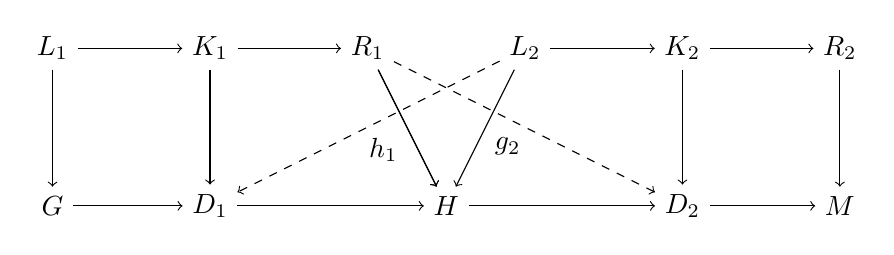
\begin{tikzpicture} 
        % Define nodes
        \node (L1) at (0,2) {$L_1$};
        \node (K1) at (2,2) {$K_1$};
        \node (R1) at (4,2) {$R_1$};
        \node (L2) at (6,2) {$L_2$};
        \node (K2) at (8,2) {$K_2$};
        \node (R2) at (10,2) {$R_2$};
        \node (G) at (0,0) {$G$};
        \node (T) at (5,0) {$H$};
        \node (M) at (10,0) {$M$};
        \node (D1) at (2,0) {$D_1$};
        \node (D2) at (8,0) {$D_2$};
      
        % Draw arrows
        % Top row
        \draw[->] (L1) -- node[above] {} (K1);
        \draw[->] (K1) -- node[above] {} (R1);
        \draw[->] (L2) -- node[above] {} (K2);
        \draw[->] (K2) -- node[above] {} (R2);
      
        % Vertical arrows
        \draw[->] (L1) -- node[left] {} (G);
        \draw[->] (R1) -- node[right] {} (T);
        \draw[->] (R2) -- node[right] {} (M);
        \draw[->] (K1) -- node[right] {} (D1);
        \draw[->] (K2) -- node[right] {} (D2);
      
        % Bottom row
        \draw[->] (G) -- node[below] {} (D1);
        \draw[->] (D1) -- node[below] {} (T);
        \draw[->] (T) -- node[below] {} (D2);
        \draw[->] (D2) -- node[below] {} (M);

        \draw[->,dashed] (R1) -- node[below] {} (D2);
        \draw[->,dashed] (L2) -- node[below] {} (D1);
      
        % Diagonal arrows
        \draw[->] (R1) -- node[below left] {$h_1$} (T);
        \draw[->] (L2) -- node[below right] {$g_2$} (T);
      \end{tikzpicture}
\end{definition}

\begin{definition}[Sequential critical pair]
    Let $r_i \colon \langle L_i \leftarrow K_i \rightarrow R_i \rangle$ be rules, for $i = 1, 2$. A pair of direct derivations $G \Rightarrow_{r_1} H \Rightarrow_{r_2} M$ as depicted below is a sequential critical pair if the following holds.
    \begin{itemize}
        \item Minimality:$H = h_1(R_1) \cup g_2(L_2)$.
        \item Conflict: The steps are not sequentially independent.
    \end{itemize}
    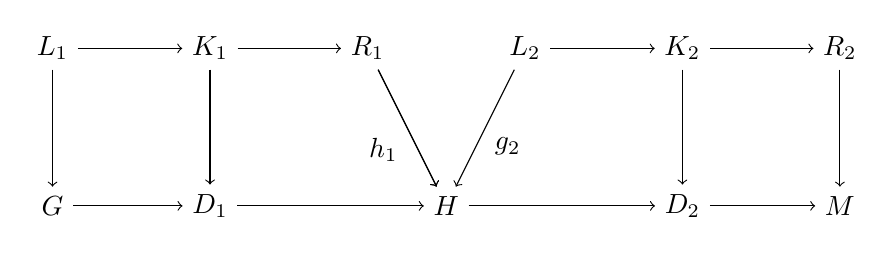
\begin{tikzpicture} 
        % Define nodes
        \node (L1) at (0,2) {$L_1$};
        \node (K1) at (2,2) {$K_1$};
        \node (R1) at (4,2) {$R_1$};
        \node (L2) at (6,2) {$L_2$};
        \node (K2) at (8,2) {$K_2$};
        \node (R2) at (10,2) {$R_2$};
        \node (G) at (0,0) {$G$};
        \node (T) at (5,0) {$H$};
        \node (M) at (10,0) {$M$};
        \node (D1) at (2,0) {$D_1$};
        \node (D2) at (8,0) {$D_2$};
      
        % Draw arrows
        % Top row
        \draw[->] (L1) -- node[above] {} (K1);
        \draw[->] (K1) -- node[above] {} (R1);
        \draw[->] (L2) -- node[above] {} (K2);
        \draw[->] (K2) -- node[above] {} (R2);
      
        % Vertical arrows
        \draw[->] (L1) -- node[left] {} (G);
        \draw[->] (R1) -- node[right] {} (T);
        \draw[->] (R2) -- node[right] {} (M);
        \draw[->] (K1) -- node[right] {} (D1);
        \draw[->] (K2) -- node[right] {} (D2);
      
        % Bottom row
        \draw[->] (G) -- node[below] {} (D1);
        \draw[->] (D1) -- node[below] {} (T);
        \draw[->] (T) -- node[below] {} (D2);
        \draw[->] (D2) -- node[below] {} (M);

        % \draw[->,dashed] (R1) -- node[below] {} (D2);
        % \draw[->,dashed] (L2) -- node[below] {} (D1);
      
        % Diagonal arrows
        \draw[->] (R1) -- node[below left] {$h_1$} (T);
        \draw[->] (L2) -- node[below right] {$g_2$} (T);
      \end{tikzpicture}
\end{definition}

\begin{theorem}
    \todo{rewrite}
    Let $\langle \Sigma, \mathcal{R} \rangle$ and $\langle \Sigma, \mathcal{S} \rangle$ be terminating hypergraph transformation systems. If there are no sequential critical pairs of shape $S \Rightarrow_{\mathcal{R}} T \Rightarrow_{\mathcal{S}} U$, then the combined system $\langle \Sigma, \mathcal{R} \cup \mathcal{S} \rangle$ is terminating.
\end{theorem}

    % %     \subsection{Forward Closure Method of DPO GRS}  
    % %     \label{sec:forward_closure}
    % %     Plump \cite{Plump1995} introduced a necessary and sufficient termination condition for left-injective DPO hypergraph rewriting via forward closure, though verifying this condition is undecidable.


\begin{definition}[Instance]
    \todo{rewrite}
    Consider a finite or infinite derivation
    

    \begin{tikzpicture}
      % Nodes
      \node (pi1) at (0,0) {$\pi_1$};
      \node (pip1) at (2,0) {$\pi'_1$}; 
      \node (pi2) at (4,0) {$\pi_2$};
      \node (pip2) at (6,0) {$\pi'_2$};
      \node (pi3) at (8,0) {$\pi_3$};
      \node (pip3) at (10,0) {$\pi'_3$};
      \node (dots) at (12,0) {$\dots$};
    
      % Horizontal arrows in the top row
      \draw[->] (pi1) -- ++(-2,0);
      \draw[->] (pip1) -- ++(2,0);
      \draw[->] (pi2) -- ++(-2,0);
      \draw[->] (pip2) -- ++(2,0);
      \draw[->] (pi3) -- ++(-2,0);
      \draw[->] (pip3) -- ++(2,0);
    
      % Vertical arrows
      \draw[->] (pi1) -- ++(0,-1);
      \draw[->] (pip1) -- ++(0,-1);
      \draw[->] (pi2) -- ++(0,-1);
      \draw[->] (pip2) -- ++(0,-1);
      \draw[->] (pi3) -- ++(0,-1);
      \draw[->] (pip3) -- ++(0,-1);
    
      % Diagonal arrows
      \draw[->] (pip1) -- ++(1,-1);
      \draw[->] (pip2) -- ++(1,-1);
      \draw[->] (pip3) -- ++(1,-1);
    
      % Horizontal arrows in the bottom row
      \draw[->] (pi1) -- ++(2,0);
      \draw[->] (pip1) -- ++(-2,0);
      \draw[->] (pi2) -- ++(2,0);
      \draw[->] (pip2) -- ++(-2,0);
      \draw[->] (pi3) -- ++(2,0);
      \draw[->] (pip3) -- ++(-2,0);
    \end{tikzpicture}
    
    A derivation is an \textit{instance} (or \textit{embedding}) of this derivation if it can be written
    

    
    where for each $i \mathop{\geq} 1$, $\phi_i$ and $\phi'_i$ are pushouts with injective vertical morphisms. (So the pushouts constituting the derivation are composed of the pushouts $\pi_i$ and $\phi_i$, respectively $\pi'_i$ and $\phi'_i$.)
\end{definition}

\begin{definition}[forward closure]
    Forward closures are inductively defined as follows:
    \begin{enumerate}
        \item Every direct derivation $L \mathop{\Rightarrow}_{r,g} R$ with surjective $g$ is a forward closure.
        \item A derivation $G \mathop{\Rightarrow}^+ H \mathop{\Rightarrow} M$ is a forward closure if $G \mathop{\Rightarrow}^+ H$ is an instance of a forward closure, and $H \mathop{\Rightarrow} M$ is a direct derivation such that
        \begin{itemize}
            \item $G \mathop{\Rightarrow}^+ H$ and $H \mathop{\Rightarrow} M$ are dependent,
            \item $\text{New}(H) \mathop{\subseteq} \text{Redex}(H \mathop{\Rightarrow} M)$.
        \end{itemize}
    \end{enumerate}
\end{definition}

\begin{definition}[infinite forward closure]
    \todo{rewrite}
    An \textit{infinite forward closure} is an infinite derivation $G_0 \mathop{\Rightarrow} G_1 \mathop{\Rightarrow} G_2 \mathop{\Rightarrow} \dots$ that contains a forward closure as a prefix. That is, there is some $n \mathop{\geq} 1$ such that $G_0 \mathop{\Rightarrow}^+ G_n$ is a forward closure.
\end{definition}

\begin{definition}[Consumptive System]
    \todo{rewrite}
    A graph rewriting system is \textit{consumptive} if each rule $(L \mathop{\leftarrow} K \mathop{\rightarrow} R)$ has a non-surjective morphism $K \mathop{\to} L$.
\end{definition}
    
\begin{theorem}[Main Theorem]
    \todo{rewrite}
    A graph rewriting system is terminating if, and only if, it is consumptive and does not admit an infinite forward closure.
\end{theorem}
    % %     \subsection{Termination Criterion of injective DPO GRS based on E-dependency relation \textcolor{red}{todo}} 
    % \begin{definition}[E-graph]
\end{definition}

\begin{definition}[size of a graph]
\end{definition}

\begin{definition}[production]
\end{definition}

\begin{definition}[E-concurrent production~\text{\cite[Def~3.1]{LEVENDOVSZKY200787}}]
    An E-concurrent production $p^*$ is an E-based composition if there is at least one input graph $G_0$ with an E-related transformation $G_0 \xrightarrow{p^*} H$.
\end{definition}

\begin{definition}[E-dependency relation~\text{\cite[Def~3.2]{LEVENDOVSZKY200787}}]
    Consider a possibly infinite sequence of graph productions $p_i$, ($i \mathop{=} 1, 2, \ldots$) and a sequence of E-dependency relations $((E_i, e_i^*, e_{i+1}))$ leading to a sequence of their E-based compositions $(p_i^* \mathop{=} (L_i^* \mathop{\leftarrow} K_i^* \mathop{\rightarrow} R_i^*))$ with $p_1^* \mathop{=} p_1$ and $p_n^* \mathop{=} (p_1 *_{E_1} p_2) *_{E_2} \ldots *_{E_n} p_n$.
    
    A cumulative LHS series of this sequence is the graph series $L_n^*$ consisting of the left-hand side graphs of $p_n^*$. Moreover, a cumulative size series of a production sequence is the nonnegative integer series $|L_n^*|$.
    \end{definition}

\begin{theorem}[Termination~\cite{LEVENDOVSZKY200787}]
    A \text{GTS} $= (P)$ (Def.??) terminates if for all infinite cumulative LHS sequences $(L_i^*)$ of the graph productions created from the members of $P$, it holds that
    \[
    \lim_{i \mathop{\to} \infty} |L_i^*| \mathop{=} \infty.
    \]
    Note that we assume finite input graphs and injective matches.
\end{theorem} 
    %     \subsection{Type Graph Method for DPO GRS}
    %     \label{sec:type_graph_method}
    %         \subsubsection{Well-founded semirings}
    %         \begin{definition}[Monoid]
    \label{def:monoid}
    \todo{to check and add reference}
    A \textbf{monoid} is a triple \(\langle S, \cdot, e \rangle\) where \(S\) is a set, \(\cdot : S \times S \to S\) is a binary operation and \(e \in S\) is constant
    satisfying for all \(a, b, c \in S\):
    \begin{itemize}
        \item \textbf{Associativity}: \((a \cdot b) \cdot c = a \cdot (b \cdot c)\),
        \item \textbf{Identity}: \(a \cdot e = a = e \cdot a\).
    \end{itemize}
    The monoid is \textbf{commutative} if \(a \cdot b = b \cdot a\) for all \(a, b \in S\).
\end{definition} 

\begin{definition}[Semiring]
    \label{def:semiring}
    \todo{to check and to add some references}
    A \textbf{semiring} is a tuple \(\langle S, \oplus, \odot, 0, 1 \rangle\) where:
    \begin{itemize}
        \item  \(\langle S, \oplus, 0 \rangle\) forms a commutative monoid,
        \item  \(\langle S, \odot, 1 \rangle\) forms a monoid,
        \item  $0$ is an annihilator for $\odot$ : For all \(a \in S\),
              \(
                  0 \odot a = 0 = a \odot 0
              \),
        \item $\odot$ distributes over $\oplus$: For all \(a, b, x \in S\),
              \begin{itemize}
                \item $(a \oplus b) \odot x = (a \odot x) \oplus (b \odot x)$
                \item $x \odot (a \oplus b) = (x \odot a) \oplus (x \odot b)$
              \end{itemize}                 
    \end{itemize}
    The semiring is \textbf{commutative} if its multiplicative monoid \(\langle S, \odot, 1 \rangle\) is commutative.
\end{definition}


\begin{definition}[Well-founded semiring]
    \label{def:well_founded_semiring}
    A \textbf{well-founded semiring} is a tuple \(\langle S, \oplus, \odot, 0, 1, \prec, \leq \rangle\) where:
    \begin{itemize}
        \item  \(\langle S, \oplus, \odot, 0, 1 \rangle\) is a semiring,
        \item \textbf{Order Relations}: 
            \begin{itemize}
                \item \(\prec, \leq \subseteq S \times S\) are non-empty orders,
                \item \(\prec \subseteq \leq\) (i.e., \(x \prec y \implies x \leq y\)),
                \item \(\leq\) is reflexive.
            \end{itemize}
    \end{itemize}
    The structure satisfies:
    \begin{itemize}
        \item \(\text{SN}(\succ / \geq)\) (strong normalization modulo \(\geq\)),
        \item \(0 \neq 1\),
        \item For all \(x, x', y, y' \in S\):
            \begin{align*}
                x \leq x' \land y \leq y' &\implies x \oplus y \leq x' \oplus y' \tag{S1} \label{ax:S1} \\
                x \prec x' \land y \prec y' &\implies x \oplus y \prec x' \oplus y' \tag{S2} \label{ax:S2} \\
                x \leq x' \land 1 \leq y &\implies x \odot y \leq x' \odot y \tag{S3} \label{ax:S3} \\
                x \prec x' \land 1 \leq y \neq 0 &\implies x \odot y \prec x' \odot y \tag{S4} \label{ax:S4}
            \end{align*}
    \end{itemize}
    The semiring is \textbf{strictly monotonic} if it additionally satisfies:
    \[
        x \prec x' \land y \leq y' \implies x \oplus y \prec x' \oplus y' \tag{S5} \label{ax:S5}
    \]
\end{definition}

\begin{example}[Semiring examples~\text{\cite[Ex. 2.7]{endrullis2024generalized}}]
    \label{ex:semiring_examples}
    \textbf{Arithmetic semiring}: \(\langle \mathbb{N}, +, \cdot, 0, 1, <, \leq \rangle\) is strictly monotonic and well-founded.

    \textbf{Tropical semiring}: \(\langle \mathbb{N} \cup \{\infty\}, \min, +, \infty, 0, <, \leq \rangle\) is well-founded but not strictly monotone.

    \textbf{Arctic semiring}: \(\langle \mathbb{N} \cup \{-\infty\}, \max, +, -\infty, 0, <, \leq \rangle\) is well-founded but not strictly monotone.
\end{example}
    %         \subsubsection{Weighted Type Graphs}
    %         The following definition of a weighted type graph is obtained from~\cite[\textdef~3.1]{endrullis2024generalized}.
\begin{definition}[Weighted Type Graph]
    \label{def:weighted_type_graph}
    A \textbf{weighted type graph} \(\mathcal{T} \mathop{=} (T, \mathbb{E}, \mathcal{S}, w)\) consists of:
    \begin{itemize} 
        \item An object \(T \mathop{\in} \mathcal{C}_0\), called the \textbf{type graph},
        \item A set \(\mathbb{E}\) of arrows \(e \mathop{\in} \mathcal{C}_1\) with \(\operatorname{codom}(e) \mathop{=} T\), called the \textbf{\(T\)-valued elements},
        \item A well-founded, commutative semiring \(\mathcal{S}=\langle S, \mathop{\oplus}, \mathop{\odot}, 0, 1, \prec, \leq \rangle \),
        \item A weight function \(w : \mathbb{E} \mathop{\to} S \mathop{\setminus} \{0_S\}\).
    \end{itemize}
    \(\mathcal{T}\) is \textbf{finitary} if for every \((e:X \mathop{\to} T) \mathop{\in} \mathbb{E}\) and every \(G \mathop{\in} \mathcal{C}_0\), the sets \(\operatorname{Hom}(X, G)\) and \(\operatorname{Hom}(G, T)\) are finite.
\end{definition}
\todo{include : $weighted_type_graph_remark_geq1$}
\todo{include : $weighted_type_graph_remark_neq0$}
    %         \subsubsection{Weighing Morphisms and Objects}
    %         \input{sections/endrullis_graph_weight}
    %         \subsubsection{Estimating Weight Changes}
    %         \input{sections/endrullis_weighing_pushout_objects}
    %         % \subsection{Decreasing Rule}
    %         \todo{to be weakened to the original version by endrullis}
\todo{maybe add the core lemma for estimating pushout object weight, but adapt to estimating DPO objects weight difference}
\begin{definition}[Decreasing Rules~\text{\cite[\textdef~5.9]{endrullis2024generalized}}]
    \label{def:decreasing_rule}
    Let $\mathcal{T} = (T,\mathbb{E},\mathcal{S}, w)$ be a finitary weighted type graph where $\mathcal{S}=\langle S, \oplus, \odot, 0, 1, \prec, \leq \rangle$ is a well-founded, commutative, \(\mathfrak{F}\) a DPO rewriting framework, $\rho = (L \overset{l}{\leftarrow} K \overset{r}{\rightarrow} R)$ a DPO rewriting rule. 

    \noindent
    The rule $\rho$ is \textbf{weakly decreasing} w.r.t. $\mathcal{T}$ in $\mathfrak{F}$ if 
            for every $t_K : K \to T$,
                $$ 
                  w_\mathcal{T}(\{l \star - = t_K\}) \succeq w_\mathcal{T}(\{r\star - = t_K\})$$
           
    \noindent
    The rule $\rho$ is \textbf{uniformly decreasing} w.r.t. $\mathcal{T}$ in $\mathfrak{F}$ if
        \begin{itemize}
            \item[]- there exists a context closure $c_\rho$ for $\rho$ and $\mathcal{T}$ in $\mathfrak{F}$, and
            \item[]- for every $t_K : K \to T$,
            \begin{itemize}
                \item[] $\bullet$ $\{l \star - = t_K\} = \emptyset = \{r \star - = t_K\}$, or
                \item[] $\bullet$ $w_\mathcal{T}(\{l \star - = t_K\}) \succ    w_\mathcal{T}(\{r \star - = t_K\}) + \delta$.
            \end{itemize}
        \end{itemize}  
         
    \noindent
    The rule $\rho$ is
            \textbf{$\delta$-closure decreasing} w.r.t. $\mathcal{T}$ in $\mathfrak{F}$ if the following hold:
            \begin{itemize}
                \item[]- $S$ is strictly monotonic semiring,
                \item[]- $\rho$ is weakly decreasing,
                \item[]- there exists a context closure $c_\rho$ for $\rho$ and $\mathcal{T}$ in $\mathfrak{F}$,
                \item[]- $w_\mathcal{T}(\{l \star - = t_K\}) \succ  w_\mathcal{T}(\{r \star - = t_K\})$ for $t_K = l \star c_\rho$.
            \end{itemize}
\end{definition}

The following lemma states that decreasing rules reduce the weights of host graphs, provided specific constraints are satisfied.
\begin{lemma}[Decreasing steps~\text{\cite[Theorem C.3]{endrullis2024generalized}}]
    \label{lem:decreasing_step}
    \ \newline 
\begin{minipage}{0.7\textwidth}
    Let $\mathcal{T} = (T,\mathbb{E}, \mathcal{S}, w)$ be a finitary weighted type graph where $\mathcal{S} = \langle S, \oplus, \odot, 0, 1, \prec, \leq \rangle$ is a strong monotonic, commutative semiring, $\rho$ a rewriting rule and $\Delta \in \mathfrak{F}(\rho)$ a DPO diagram
    (shown on the right)   such that the following conditions hold:
\end{minipage}  
\begin{minipage}{0.3\textwidth}
    \begin{center}
        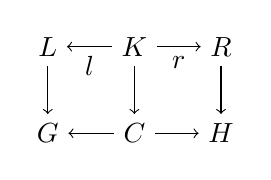
\begin{tikzpicture}[node distance=11mm]
          \node (I) {$K$};
          \node (L) [left of= I] {$L$};
          \node (R) [right of=I] {$R$}; 
          \node (G) [below of=L] {$G$};
          \node (C) [below of=I] {$C$};
          \node (H) [below of=R] {$H$};
        %   \node (T) [left=of $(L)!0.5!(G)$] {$T$};
        %   \draw [->] (L) to  node [label, above] {$c$}  (T);
        %   \draw [->] (G) to  node [label, below] {$\alpha$} (T);
          \draw [->] (I) to node [label, below] {$l$} (L);
          \draw [->] (I) to node [label, below] {$r$} (R);
          \draw [->] (L) to  (G);
          \draw [->] (I) to (C);
          \draw [->] (R) to (H);
          \draw [->] (C) to (G);
          \draw [->] (C) to (H);
        \end{tikzpicture}
      \end{center}
\end{minipage}
   \begin{itemize}
       \item $\operatorname{left}(\Delta)$ is weighable with \(\mathcal{T}\), and
       \item $\operatorname{right}(\Delta)$ is bounded above by \(\mathcal{T}\), and
       \item $w(e) \succeq 1_S$ for all $e \in \mathbb{E}$.
   \end{itemize}

   \noindent
  We have:
   \begin{itemize}
       \item $w_\mathcal{T}(G) \succeq w_\mathcal{T}(H)$ if $\rho$ is weakly decreasing,
       \item $w_\mathcal{T}(G) \succ w_\mathcal{T}(H)$ if $w(e) \succeq 1_S$ for all $e \in \mathbb{E}$, and $\rho$ is uniformly or closure decreasing.
   \end{itemize}
\end{lemma} 
\begin{proof}
   See the \hyperref[proof:decreasing_step]{Appendix}.
\end{proof} 
    %         \subsubsection{Termination Criterion} 
    %         \todo{to be weakened to the original version by endrullis}
Finally, a termination criterion can be established.
\begin{theorem}[Termination~\text{\cite[Theorem 5.11]{endrullis2024generalized}}] 
    \label{thm:termination_grs}
    Let $\mathcal{A}$ and $\mathcal{B}$ be sets of DPO rewriting rules, $\mathcal{T} \mathop{=} (T,\mathbb{E}, \mathcal{S}, w)$ be a finitary weighted type graph where $\mathcal{S} \mathop{=} \langle S, \mathop{\oplus}, \mathop{\odot}, 0, 1, \prec, \leq \rangle$ is a strong monotonic, commutative semiring and $\mathfrak{F}$ a DPO rewriting framework such that

     \begin{enumerate}
        \item\label{thm1:hyp3} $w(e) \mathop{\succeq} 1_S$ for all $e \mathop{\in} \mathbb{E}$,
        % \item\label{thm1:hyp4} $\{s \mathop{\in} S\mid 1_S \leq s \mathop{\neq} 0_S\} \mathop{\subseteq} \mathbb{R}_{>0}$ 
        % \item\label{thm1:hyp4} for all $x \mathop{\in} S$, if $ 1_S \mathop{\preceq} x \mathop{\neq} 0_S$ then $\mu(x) \mathop{\geq} \mu(1_S)$ and $\mu(x) \mathop{\in} \mathbb{R}$,
        % \item\label{thm1:hyp4} for all $x \mathop{\in} S$, if $ 1_S \mathop{\preceq} x \mathop{\neq} 0_S$ then $\mu(x) \mathop{\geq} \mu(1_S)$ and $\mu(x) \mathop{\in} \mathbb{R}$,
        \item for every rule $\rho \mathop{\in} (\mathcal{A }\mathop{\cup} \mathcal{B })$ and every double pushout diagram  
        $\Delta \mathop{\in} \mathfrak{F}(\rho)$ 
        \begin{itemize}
            \item \(\operatorname{left}(\Delta)\) is weighable with \(\mathcal{T}\), and
            \item \(\operatorname{right}(\Delta)\) is bounded above by \(\mathcal{T}\). 
        \end{itemize}
    \end{enumerate}       

    \noindent If the following conditions hold:
    \begin{enumerate}
        \item either every $\rho \mathop{\in} \mathcal{A}$ is uniformly decreasing, or every $\rho \mathop{\in} \mathcal{A}$ is closure decreasing,
        \item every rule $\rho \mathop{\in} \mathcal{B}$ is weakly decreasing,
    \end{enumerate}
    then $\mathop{\Rightarrow}_{\mathcal{A},\mathfrak{F}}$ is \textbf{terminating} relative to $\mathop{\Rightarrow}_{\mathcal{B},\mathfrak{F}}$.
\end{theorem} 
\begin{proof}
    See the 
    % \hyperref[proof_termination_grs]{Appendix}.
    ref
\end{proof}
    %     \subsection{Subgraph Counting}  
    %     The subgraph-counting method in 2024 lmcs by Overbeek and Endrullis is designed for the PBPO+ 2023 pbpo+ ref —a rewriting formalism capable of simulating left-injective DPO rewriting.
    %     \subsection{Termination Criterion for DPO GRS with NAC}
    %     \begin{definition}
    Let $V_L$ be the set of nodes in $L$, and $M_L \mathop{=} \{m_1, \dots, m_r\}$ the set of matches $m_i : V_L \mathop{\to} V_L$ of $V_L$ into itself, including the identity $id_{V_L} \mathop{=} m_1$. We construct a Labelled Transition System $\mathcal{L}^p \mathop{=} (S, \Lambda, \longrightarrow)$ as follows:

    \begin{enumerate}
        \item $S$ contains a state $s_i$ for each graph 
        $H_i^p \mathop{\in} \mathfrak{H}_p^p$. 
        % $H_i^p \mathop{\in} \mathscr{H}$.
         Each $s_i$ induces a classification function $c_i$ for matches of $p$ such that $c_i(m_l) \mathop{=} \text{true}$ iff $m_l$ can be extended to a match on $H_i^p$, but not to a match on any other 
         $H_j^p \mathop{\in} \mathfrak{H}_p^p \mathop{\setminus} (\{H_1^p, H_i^p\} \mathop{\cup} \{H_t^p \mathop{\mid} \exists h_t^i : H_t^p \mathop{\to} H_i^p\})$,
          i.e., $H_i^p$ is the biggest graph to which $m_l$ can be extended.
        
        \item $\Lambda$ contains a label $p^i$, $i \mathop{=} 1, \dots, r$ for each morphism in $M_L$.
        
        \item The transition relation $\longrightarrow \mathop{\subseteq} S \mathop{\times} \Lambda \mathop{\times} S$ is such that $(s_i, p^l, s_j) \mathop{\in} \longrightarrow$ (denoted by $s_i \xrightarrow{p^l} s_j$) if applying $p$ with match $m_l$ on graph $H_i^p$ produces a graph for which $c_j(m_l) \mathop{=} \text{true}$.
    \end{enumerate}
\end{definition} 

\begin{definition}
    In order to consider the variation on the number of possible matches induced by the application of $p$ on the minimal context for a given state, let $@|\cdot|: S \mathop{\to} \mathbb{N}$ be a function which associates with each state $s_i$ the number of matches for $p$ on the graph $H_i^p$ prior to application of $p$, and with $|\cdot|: S \mathop{\to} \mathbb{N}$ the function defining the number of matches on $H_i^p$ after the application of $p$.
\end{definition}

\begin{definition}
    Let $\rho$ be a graph rewriting rule. We say that $\rho$
    \begin{itemize}
        \item \emph{must terminate} if it should terminate simply and for all transitions $s_i \xrightarrow{p_l} s_j$ and all states $s_h \mathop{\neq} s_i, s_j, s_k$, we have $\left| s_i \right| < @ | s_i |$, $\left| s_j \right| \leq @ | s_j |\mathop{+}1$ and $\left| s_h \right| \leq @ | s_h |$.
        \item \emph{may terminates} if it may terminate simply and for all states on the path the same condition on matches as above applies.
        \item \emph{does not terminate} if (it does not terminate simply AND for all states from which $s_k$ is reachable, there is a state for which the number of matches increases for some transition leading to $s_k$ increases) OR (it should or may terminate simply, but there is at least one state $s_i$ on a path from $s_1$ to $s_k$ for which $\left| s_i \right| \mathop{\geq} @ | s_i |$, for a transition reachable from state $s_i$).
    \end{itemize}
\end{definition}

\begin{theorem}[Termination~\text{\cite[Theorem~2]{bottoni2010atermination}}]
    \todo{rewrite}
    Let $@|\cdot|: S \mathop{\to} \mathbb{N}$ and $|\cdot|: S \mathop{\to} \mathbb{N}$ be counting functions as defined above, let $p$ be a rule, and let $G$ be a finite graph. Then the following holds:
    \begin{enumerate}
        \item If rule $p$ is of type \textbf{must terminate}, then the application of \texttt{asLongAsPossible $p$ end} on the starting graph $G$ terminates after a finite number of steps.
        
        \item If $p$ is of type \textbf{does not terminate}, then the application of \texttt{asLongAsPossible $p$ end} on the starting graph $G$ does not terminate.
    \end{enumerate}
\end{theorem}   
    \section{Morphisms of Graph Rewriting Systems}
        \label{sec:morphisms_from_dpo_to_pbpop}
        \subsection{Morphism from left-injective DPO GRS with injective match to PBPO+}
        \label{sec:morphism_from_dpo_grs_to_pbpop}
        \begin{example}[ \cite{overbeek2023pbpo_JLAMP}]
            In the category of unlabeled directed graphs, there exists a mono-partial morphism classifier $(T,\eta)$ where 
            \begin{itemize}
                \item for all unlabeled graph $G=(V,A,s,t)$, we have $T(G) \mathop{=} (V_*,E_*,s_*,t_*)$ where $V_* \mathop{=} V \uplus \{*\}, E_* \mathop{=} E \uplus (V_* \mathop{\times} V_x), s_*(e) \mathop{=} s(e)$ if $e \mathop{\in} E$ and $\pi_1(e)$ otherwise, and $t_*(e) \mathop{=} t(e)$ if $e \mathop{\in} E$ and $\pi_2(e)$ otherwise.
            \end{itemize}
            An example is given by 
            \begin{center}
                $G \; \mathop{=} $
                \begin{tikzcd}
                v \arrow[loop, distance=2em, in=215, out=145] \arrow[rr] &  & w
                \end{tikzcd}
                \quad and \quad 
                $T(G) \; \mathop{=} \hspace{-3mm} $ % https://tikzcd.yichuanshen.de/#N4Igdg9gJgpgziAXAbVABwnAlgFyxMJZABgBpiBdUkANwEMAbAVxiVpAF9T1Nd9CUAJnJVajFmwDunbiAzY8BIgEZSy0fWatEIADq6ARhBydRMKAHN4RUADMAThAC2SMiBwRX1BhAhoiggDsZLaMcDCiDHQGMAwACryKAiD2WBYAFiZcdo4uiG4eSMrZIA7OXu6eiMIgDFhg2iBQxjjmINQxYFBIALQAzMQlZXk1hYiqtfWNzTit3UO5SKNVNT5+RCFhEd7RsQkK-GypGSbeU2wzczI55ePUYxNr-igAnJsM4ZG78YmHOseZdqTBoXFptBa3ApVNxPALBUihD7bWrffZ8JT-NKAs4gnSXcGyYYVB4dGBdJADHHTMHzQmLO6VCqdbqISnA6mzAk3Eb3aFU0Gc2ncoq8pak8msmHnPE00wcIA
                \begin{tikzcd}
                v \arrow[loop, distance=2em, in=215, out=145] \arrow[rr] \arrow[rd, dotted, bend right] \arrow[dotted, loop, distance=4em, in=240, out=140, looseness=3] \arrow[rr, dotted, bend left] &                                                                                                & w \arrow[dotted, loop, distance=2em, in=35, out=325] \arrow[ll, dotted, bend left] \arrow[ld, dotted, bend left] \\
                                                                                                                                                                  & \mathop{\star} \arrow[ru, dotted] \arrow[dotted, loop, distance=2em, in=305, out=235] \arrow[lu, dotted] &                                                                                                       
                \end{tikzcd},
            \end{center}
        
            where the dotted edges represent the edges $e \mathop{\in} V_\star \mathop{\times} V_\star$.
            It can be seen that for any partial homomorphism $\psi: H \mathop{\to} G$ defined on subgraph $H' \mathop{\subseteq} H$, there exists exactly one homomorphism $\psi_\star : H \mathop{\to} T(G)$ such that $\psi_\star(x) \mathop{=} \psi(x)$ for $x \mathop{\in} V_{H'} \mathop{\cup} E_{H'}$ and $\psi_\star(x) \notin V_{G} \mathop{\cup} E_{G}$ for $x \notin V_{H'} \mathop{\cup} E_{H'}$. Equivalently, $\psi_\star$ is the unique morphism $\varphi_{m,f} : H \mathop{\to} T(G)$ making
                \begin{center}
                    % https://tikzcd.yichuanshen.de/#N4Igdg9gJgpgziAXAbVABwnAlgFyxMJZABgBpiBdUkANwEMAbAVxiRAA0QBfU9TXfIRQBGclVqMWbAELdeIDNjwEiZYePrNWiEAEE5fJYKKj11TVJ0AVABTSAlN3EwoAc3hFQAMwBOEALZIoiA4EEgAzNQ4dFgMbAAWEBAA1iDmktogADpZMNEA+rLUDHQARjAMAAr8ykIgWGDYsAYgvgFIZCFhiABMUTFxOokpaRJabIHFZRXVRio6DU2sPN5+gYidoUHp4zpeoyXlVTXGC41YzSuta0h9XRE7ltlZaHQ+AMYlcHDA-lzAXi4B2mxzmdUWF2WFC4QA
                    \begin{tikzcd}[column sep=15mm]
                    H' \arrow[d, "m" description, hook] \arrow[r, "f" description] & G \arrow[d, "\eta_G" description, hook] \\
                    H \arrow[r, "\varphi_{m,f}" description]                    & T(G)                                   
                    \end{tikzcd}
                \end{center}
            a pullback square, where $H \stackrel{m}{\hookleftarrow} H' \stackrel{f}{\to} G$ a partial map span representation of $\psi$, and $\eta_G$ and $m$ are inclusions.
            
            The generalization to labeled graphs is straightforward: between any two nodes $u,v \mathop{\in} V_\star$ and for every label $l$, there is one $l$-labeled edge representing an undefined $l$-edge between $u$ and $v$.
        \end{example}
        
        The following theorem is an instance of \cite[Definition 71]{overbeek2023pbpo_JLAMP}.
        \begin{definition}
            Let $L \overset{l}{\leftarrowtail} K \overset{r}{\rightarrowtail} R$ be a DPO graph rewriting rule. The diagram depicted below where the left square a pushout (which is also a pullback) is a $\mathbf{PBPO}^+$ rule, denoted $|\rho|$.
        \[ 
        \begin{tikzcd}
        L \arrow[r, "l"] & K \arrow[r, "r"] & R \\
        L' \arrow[u, "\eta_L", hook] \arrow[r, "l'"'] & T(K) \arrow[u, "\eta_K"', hook]
        \end{tikzcd}
        \]
        
        
        \end{definition} 
        
        The following theorem is an instance of \cite[Theorem 72]{overbeek2023pbpo_JLAMP}.
        \begin{theorem}
            In $\mathbf{Graph}$.
            
            let $\mathrm{DPO}$ be the DPO graph rewriting system with injective matches.
        
            For any left-injective DPO rule $\rho$, $|\rho|$ is a well-defined $\mathrm{PBPO}^+$ rule. 
            
            For any $G \mathop{\to} ^{\rho}_{\mathrm{DPO}} H$, we have $G \mathop{\to} ^{|\rho|}_{\mathrm{PBPO}^+} H$.  
        \end{theorem}
        \begin{proof}
            \todo{todo}
        \end{proof}
        